\documentclass[a4paper,12pt]{article} % добавить leqno в [] для нумерации слева
\usepackage[a4paper,top=1.3cm,bottom=2cm,left=1.5cm,right=1.5cm,marginparwidth=0.75cm]{geometry}
%%% Работа с русским языком
\usepackage{cmap}					% поиск в PDF
\usepackage[warn]{mathtext} 		% русские буквы в фомулах
\usepackage[T2A]{fontenc}			% кодировка
\usepackage[utf8]{inputenc}			% кодировка исходного текста
\usepackage[english,russian]{babel}	% локализация и переносы
\usepackage{physics}
\usepackage{multirow}

%%% Нормальное размещение таблиц (писать [H] в окружении таблицы)
\usepackage{float}
\restylefloat{table}


\usepackage{graphicx}

\usepackage{wrapfig}
\usepackage{tabularx}

\usepackage{hyperref}
\usepackage[rgb]{xcolor}
\hypersetup{
	colorlinks=true,urlcolor=blue
}

%%% Дополнительная работа с математикой
\usepackage{amsmath,amsfonts,amssymb,amsthm,mathtools} % AMS
\usepackage{icomma} % "Умная" запятая: $0,2$ --- число, $0, 2$ --- перечисление

%% Номера формул
%\mathtoolsset{showonlyrefs=true} % Показывать номера только у тех формул, на которые есть \eqref{} в тексте.

%% Шрифты
\usepackage{euscript}	 % Шрифт Евклид
\usepackage{mathrsfs} % Красивый матшрифт
\usepackage{pgfplots}
\pgfplotsset{compat=1.9}

%% Свои команды
\DeclareMathOperator{\sgn}{\mathop{sgn}}

%% Перенос знаков в формулах (по Львовскому)
\newcommand*{\hm}[1]{#1\nobreak\discretionary{}
	{\hbox{$\mathsurround=0pt #1$}}{}}

\date{\today}

\begin{document}

\begin{titlepage}
	\begin{center}
		{\large МОСКОВСКИЙ ФИЗИКО-ТЕХНИЧЕСКИЙ ИНСТИТУТ (НАЦИОНАЛЬНЫЙ ИССЛЕДОВАТЕЛЬСКИЙ УНИВЕРСИТЕТ)}
	\end{center}
	\begin{center}
		{\large Факультет молекулярной и химической физики}
	\end{center}
	
	
	\vspace{4.5cm}
	{\huge
		\begin{center}
			{Лабораторная работа }\\
                {"Изучение механизма окисления $LiFePO_4$ водным раствором пероксида водорода методом прямой потенциометрии".}\\
		\end{center}
	}
	\vspace{3cm}
	\begin{flushright}
		{\LARGE Работу выполнили:\\ Беляев Юрий \\ Борисов Павел  \\ Фейзрахманов Эмир \\
			\vspace{0.2cm}
			группа Б04-202}
	\end{flushright}
	\begin{flushright}
		{\LARGE Отчёт подготовил:\\ Борисов Павел  \\
			\vspace{0.2cm}
			группа Б04-202}
	\end{flushright}
	\vspace{4cm}
	\begin{center}
		\today
	\end{center}
\end{titlepage}
\section{Аннотация}
\textbf{Цель работы:} В работе изучается механизм окисления водными растворами пероксида водорода микрочастиц $LiFePO_4$. По полученным экспериментальным данным строятся кинетические кривые изменения концентрации и проводится их анализ по различным теоретическим моделям. В ходе анализа определяются константы реакций при различных значениях $pH$.
\newline \textbf{Оборудование и материалы:}
\begin{enumerate}
    \item Иономер И-160М
    \item pH-метр pH150M
    \item Магнитная мешалка
    \item Аналитические весы
    \item Секундомер
    \item Микрошпатель для порошков
    \item Мерный цилиндр или мерная колба объемом 250 мл
    \item Пластиковая емкость с крышкой объемом 1 л
    \item Стеклянный pH-чувствительный электрод
    \item Cтеклянный литий-селективный электрод
    \item Хлорсеребряный электрод сравнения
    \item Дозатор переменного объема 100-1000 мкл (2 шт.)
    \item Пластиковый наконечник с капилляром
    \item Стеклянный стакан объемом 250 мл (2 шт.)
    \item Образец $LiFePO_4$
    \item Растворы хлорида лития (1 мМ и 100 мМ)
    \item Раствор пероксид водорода (6,3 М)
    \item Гидрофосфат калия ($K_2HPO_4$)
    \item Раствор серной кислоты (1 М)
    \item Дистиллированная вода
\end{enumerate}


\section{Теоретические сведения}
\subsection{Современные химические источники тока}\par
$LiFePO_4$ является одним из наиболее перспективных материалов, являющихся вторичными химическими источниками тока, то есть способныx к восполнению потраченной энергии - \textit{циклированию}. Основой работы ХИТ является химическая реакция взаимодействия окислителя и восстановителя. Один из основных критериев оценки ХИТ – удельная энергия – определяется стандартной свободной энергией токообразующей реакции. Наибольшей теоретической удельной энергией обладают системы с литиевым анодом. \par 

Использование металлического лития приводит к тому, что свежая поверхность лития покрывается в апротонных растворителях пассивной плёнкой, которая предотвращает электронный контакт с металлической основой. Это явление приводит к тому, что при каждом заряде часть лития выбывает из дальнейшей работы. Решение этой проблемы - литий-ионные аккумуляторы, в которых отсутствует металлический литий, а процессы разряда и заряда происходят за счёт переноса ионов лития с одного электрода на другой.\par 

\begin{figure}[H]
    \centering
    \includegraphics[scale=0.12]{литий.png}
    \caption{Устройство и принцип работы литий-ионного аккумулятора
}
    \label{pic:0}
\end{figure}

В работе исследуется кинетика процесса \textit{деинтеркаляция (делитирования)} литий-железа фосфата при окислении его суспензий в растворах пероксида водорода. Изучение этого процесса помогает оптимизировать состав химических добавок для улучшения электронной проводимости. Уравнение реакции окисления $LiFePO_4$ имеет вид:
$$2LiFePO_4+H_2O_2 \rightarrow 2FePO_4 + 2LiOH$$\par 
Образующийся фосфат железа является нерастворимым в воде соединением, но в кислой среде он растворяется с образованием ионов трёхвалентного железа и фосфорной кислоты. Поэтому проведение этой реакции в данных условиях моделирует процессы, происходящие при зарядке литий-ионного аккумулятора с катодом из композита на основе $LiFePO_4$:
$$LiFePO_4 - xe^- \rightarrow Li_{(1-x)}FePO_4 + xLi^+$$\par 

\subsection{Механизм реакции}
Процесс окисления $LiFePO_4$ раствором $H_2O_2$ относится к \textit{гетерогенным гетерофазным некаталитическим} реакциям. В этом случае реагенты находятся в разном фазовом состоянии, продукты реакции также могут находиться в любом фазовом состоянии. \par 

Особенность таких реакций состоит в том, что процесс можно разделить на несколько стадий: конвективный подход реагента, адсорбция на поверхность, диффузия через пористый слой продукта реакции к ядру, химическая реакция на поверхности, диффузия по поверхности поры от ядра. Основной задачей гетерогенной кинетики является определение \textit{лимитирующей стадии} процесса и скорости всего процесса.\par 

В твердофазной реакции оценку лимитирующей стадии производят по диапазону энергии активации(области реагирования). Если лимитирующей является химическая реакция (кинетическая область реагирования) - $E_a > 40$кДж/моль. Если диффузия (диффузионная область реагирования) - $E_a < 10$ кДж/моль.\par

Характерной особенностью процесса рассматриваемой реакции является локализация реакционной зоны на поверхности раздела фаз твёрдого реагента –  $LiFePO_4$ и твёрдого продукта реакции – $FePO_4$. Такая поверхность образуется и изменяется в результате самого химического процесса, что может приводить к переходу реакции из одной макрокинетической области в другую даже при сохранении постоянными значений концентраций жидких реагентов. 

Такие реакции называются \textit{топохимическими реакциями}. Основные свойства топохимических реакций определяются тем, что реагирующие атомы или ионы, образующие кристалл, лишены той подвижности, которую они имеют в газовой или жидкой фазах. Их реакционная способность в большой степени зависит от того, в каком месте кристалла они находятся. В связи с этим, при топохимических реакциях существенное значение приобретает реальная структура кристалла, связанная с наличием в кристалле разного рода дефектов. При топохимических реакциях происходит минимальное перемещение реагирующих частиц, поэтому продукт реакции обычно сохраняет форму кристаллов исходного вещества. \par

\subsection{Уравнение Ерофеева}
Кинетика топохимической реакции хорошо описывается \textit{уравнением Ерофеева}:
\begin{equation}
    \alpha = 1- e^{-\int p dt},
\end{equation}
где $p$ - вероятность реагирования, $\alpha$ - доля прореагировавшего вещества к моменту времени $t$. Уравнение Ерофеева, приведённое к виду: 
\begin{equation}
    \alpha = 1- e^{-kt^n},
    \label{eq:erof}
\end{equation}
известно как \textit{обобщенное топокинетическое уравнение Ерофеева – Колмогорова}, где $n$ - число последовательных стадий при образовании устойчивого начального центра новой фазы, плюс постоянное число, характеризующее форму зародыша, и равное 3 при образовании сферического зародыша, 2 – цилиндрического и 1 – плоского. 

Степень отклонения $n$ от единицы характеризует меру перехода реакции в диффузионную область. Если $n>1$, то процесс находится в кинетической области, при $n<1$ - процесс в диффузионной области. В уравнении Ерофеева – Колмогорова постоянная $k$ так же зависит от $n$.

\subsection{Закон Авраами}
Другой закон зародышеобразования был предложен Авраами:
\begin{equation}
    N(t) = N_0[1-exp(-kt^n)],
\end{equation}
где $N_0$ - число потенциальных центров зародышеобразования, имеющих равную вероятность превратиться в растущий зародыш, $N(t)$ -  реальное число зародышей, образовавшееся к моменту времени $t$.

Выражение для скорости изменения степени превращения вещества ($\alpha$) в продукт новой фазы имеет вид (справедливо при малых ($\alpha$)):
\begin{equation*}
    \alpha(t) =\frac{8\pi \rho N_0\nu}{k_1^3m_0}[e^{-k_1t}-1+k_1t-\frac{(k_1t)^2}{2}+\frac{(k_1t)^3}{6}]
\end{equation*}
\subsection{Уравнение Ленгмюра}\par 
Изучаемую реакцию можно рассматривать как реакцию эквивалентного ионного обмена между $Li^+$ и $Fe^3+$. При этом значения \textit{сорбционной ёмкости} - количества вещества, которое может поглотить сорбент на единицу своей массы - зависят от времени сорбции. Изотермы катионного обмена описываются уравнением Ленгмюра:
\begin{equation}
    A_t = A_mkC_p\frac{1}{1+kC_p},
    \label{eq:sorb}
\end{equation}
где $k$ - константа Ленгмюра, $C_p$ -равновесная концентрация сорбата, $A_t$ - текущее значение сорбционной ёмкости, $A_m$ - величина сорбционной емкости в равновесных условиях.

При предположении, что количество (доля) замещенных активных центров в сорбенте зависит не только от концентрации сорбата в растворе, но и от времени сорбции, уравнение \eqref{eq:sorb} примет вид: 
\begin{equation*}
    A_t = k_1Ct(1-\frac{A_t}{A_m}).
\end{equation*}

Так же допустим, что десорбция сорбата, в отличие от допущений, принятых при выводе уравнения Ленгмюра, принята зависимой от концентрации сорбата в растворе и относительной величины сорбционной емкости сорбента:
\begin{equation*}
     A_t = k_2C\frac{A_t}{A_m}.
\end{equation*}

При таких допущениях выполняется равенство значений $A_t$ в этих уравнениях, из которого получена временная зависимость текущего значения $A_t$:
\begin{equation}
    \frac{1}{A_t} = \frac{1}{A_m} + \frac{1}{ktA_m},
    \label{eq:leng}
\end{equation}
где $k$ -константа скорости реакции ионного обмена ($c^{-1}$).

\subsection{Потенциометрический анализ}Поскольку в эксперименте для определения концентрации протонов и ионов лития используется метод потенциометрии, рассмотрим его основные теоретические положения. 

\begin{figure}[H]
    \centering
    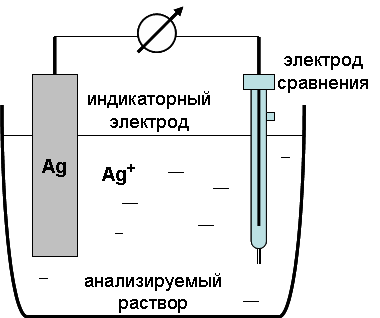
\includegraphics[scale=1]{потенц.png}
    \caption{Принцип потенциометрического анализа на примере определения концентрации ионов $Ag^{+}$ при помощи серебряного индикаторного электрода 
}
    \label{pic:00}
\end{figure}

Метод потенциометрии основан на измерении напряжения на электродах ячейки в отсутствие тока. При этом, один из электродов является индикаторным электродом, а другой – электродом сравнения. Измеряемое вольтметром напряжение на электродах ячейки в соответствии с \textit{уравнением Нернста} в общем случае равно: 
\begin{equation}
    E_{eq} = E_0 +\frac{RT}{zF}ln\frac{a_{ox}}{a_{red}}
\end{equation}
\subsection{Стеклянный электрод для измерения $pH$}
Наибольшее практическое применение для измерения $pH$ раствора нашел индикаторный стеклянный электрод, являющийся разновидностью мембранных электродов с твердой мембраной. Чаще других в паре с ним используют хлорсеребряный электрод сравнения.

\begin{figure}[H]
\centering
\begin{tabular}{ll}
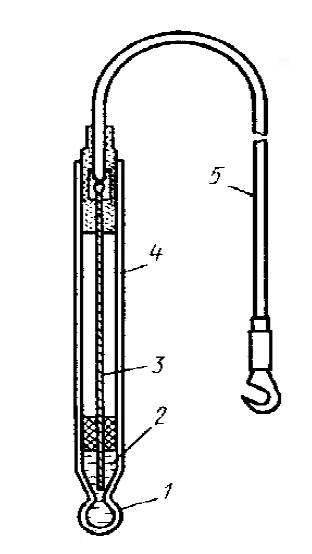
\includegraphics[width = 6cm]{pic1.png}
&
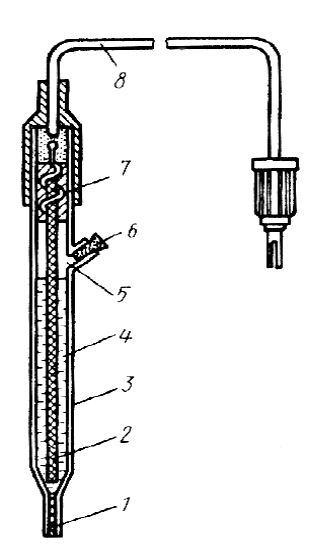
\includegraphics[width =6cm]{pic2.png}
\end{tabular}
\caption{Устройство индикаторного
стеклянного электрода (слева)
и хлорсеребряного
электрода сравнения (справа). Слева: 1 - стеклянная $pH$-чувствитеольная мембрана; 2 - 0,1 М раствор $HCL$; 3 - хлорсеребряный электрод; 4 - стеклянная трубка; 5 - контакт для подключения к $pH$-метру. Справа: 1,2 - асбестовое волокно (электролитический контакт); 3 - стеклянный корпус; 4 - насыщенный раствор $KCl$; 5,6 - отверстие для заливки раствора и пробка; 7 - серебряная проволка, покрытая $AgCl$; 8 - контакт дял подключения к прибору.}
\label{pic:000}
\end{figure}


Чувствительным элементом стеклянного электрода является шарик диаметром 15-20 мм с толщиной стенок 0,06 - 0,1 мм, изготовленной из стекла особого состава, расположенной на конце стеклянной трубки. Внутри шарика – раствор с определенным значением $pH$, в который погружен хлорсеребряный электрод сравнения. Перед работой стеклянный электрод некоторое время выдерживают в 0,1 М $HCl$. При этом ионы $H^{+}$ из раствора обмениваются на ионы $Na^{+}$ из мембраны, и в системе устанавливается равновесие. Если подготовленный таким образом электрод опустить в анализируемый раствор, содержащий ионы $H^+$, установится ионообменное равновесие между раствором и внешней поверхностью мембраны, приводящее к возникновению потенциала Нернста –  $E_1$. На внутренней поверхности стекла также возникает потенциал, $E_2$, который остается постоянным в растворе.

\subsection{Селективные электроды}
Изменяя химический состав стекла, получают ионоселективные электроды для других одновалентных ионов. Ключевым этапом подготовки электродов к работе является процедура выдерживания ионоселективного электрода в растворе соли соответствующего элемента. 

\section{Ход работы}

Задачей лабораторной работы является исследование влияния $pH$ растворов $H_2O_2$ на скорость окисления $LiFePO_4$ с целью изучения механизма данного процесса. Для этого предлагается проводить эту реакцию в буферных растворах $K_2HPO_4$ с концентрацией 5-10 мМ и значениями $pH$ в диапазоне 6-10 в режиме $pH$-статирования, реализуемого с помощью постепенного добавления раствора серной кислоты. 

Опишем последовательно этапы выполнения лабораторной работы:
\begin{enumerate}
    \item Включим иономер и pH-метр. С помощью буферного раствора 9,18 pH проведем калибровку pH-метра. Иономер был уже откалиброван.
    \item  В пластиковой емкости приготовим 1 литр 5 мМ раствора $K_2HPO_4$. Для этого взвесим m = 1,14 г вещества.
    \item С помощью мерного цилиндра отмерим 250 мл раствора $K_2HPO_4$ и перельём в отдельный стакан объемом 250 мл.
    \item Поставим стакан с раствором $K_2HPO_4$ на магнитную мешалку,опустим $pH$ метр и литий-селективный электрод.
    \item Взвесим 0,4 г $LiFePO_4$, добавим его в раствор $K_2HPO4$ и включим магнитную мешалку. Присоединим к дозатору наконечник с капилляром. С помощью дозатора с раствором серной кислоты 1 М доведем значение pH до 9,5.
    \item Наберем в дозатор ровно 1 мл 1 М раствора серной кислоты и установим дозатор в штатив с электродами. 
    \item Быстро добавляем в суспензию $LiFePO_4$ 0,25 мл 6,3 М раствора $H_2O_2$.
    \item Постепенно добавляя серную килслоту, будем удерживать нужное нам значение $pH$. С интервалом 1 минута будем записывать значения концетрации ионов лития и объема добавленной серной кислоты в течение 15 - 20 мин.
    \item Аналогичные измерения проведем для растворов с $pH$=8,5/7,5/6,5.
    \item По окончании работы промоем посуду и выключим использованные приборы.
\end{enumerate}




Полученные данные занесем в табл. \ref{tab:1},  \ref{tab:2},  \ref{tab:3}, \ref{tab:4}. Здесь $t$ - прошедшее время, $C(Li^{+})$ - показания иономера, $V(SO_4^{2-})$ - количество кислоты в дозаторе.

\begin{table}[H]
    \centering
    \begin{tabular}{|l|l|l|l|l|l|l|l|l|l|l|l|}
    \hline
        $t, \textrm{c}$& 0 & 1 & 2 & 3 & 4 & 5 & 6 & 7 & 8 & 9 & 10  \\ \hline
        $pH$ & 9,5 & 9,5 & 9,5 & 9,5 & 9,5 & 9,5 & 9,5 & 9,5 & 9,5 & 9,5 & 9,5  \\ \hline
        $C(Li^{+}), \textrm{мМ}$ & 0,383 & 0,55 & 0,717 & 0,892 & 1,024 & 1,052 & 1,3 & 1,43 & 1,54 & 1,67 & 1,75  \\ \hline
        $V(SO_4^{2-}), \textrm{мл}$ & 1000 & 915 & 855 & 810 & 770 & 735 & 700 & 675 & 645 & 610 & 590 \\ \hline
        $t, \textrm{c}$& 11 & 12 & 13 & 14 & 15 & 16 & 17 & 18 & 19 & 20 &\\ \hline
        $pH$ & 9,5 & 9,5 & 9,5 & 9,5 & 9,5 & 9,5 & 9,5 & 9,5 & 9,5 & 9,5 &   \\ \hline
        $C(Li^{+}), \textrm{мМ}$ & 1,86 & 1,96 & 2,05 & 2,15 & 2,25 & 2,31 & 2,41 & 2,48 & 2,58 & 2,62 & \\ \hline
        $V(SO_4^{2-}), \textrm{мл}$ & 565 & 545 & 520 & 500 & 480 & 465 & 440 & 430 & 405 & 400 & \\ \hline
    \end{tabular}
    \caption{Полученные данные в эксперименте с pH суспензии равной 9,5.}
	\label{tab:1}
\end{table}

\begin{table}[H]
    \centering
    \begin{tabular}{|l|l|l|l|l|l|l|l|l|l|l|l|}
    \hline
          $t, \textrm{мин}$& 0 & 1 & 2 & 3 & 4 & 5 & 6 & 7 & 8 & 9 & 10  \\ \hline
          $pH$ & 8,5 & 8,5 & 8,5 & 8,5 & 8,5 & 8,5 & 8,5 & 8,5 & 8,5 & 8,5 & 8,5  \\ \hline
       $C(Li^{+}), \textrm{мМ}$ & 0,6 & 0,837 & 1,122 & 1,35 & 1,59 & 1,79 & 1,98 & 2,18 & 2,35 & 2,51 & 2,67 \\ \hline
        $V(SO_4^{2-}), \textrm{мл}$ & 1000 & 860 & 770 & 685 & 630 & 580 & 525 & 475 & 430 & 385 & 350 \\ \hline
        $t, \textrm{мин}$&  11 & 12 & 13 & 14 & 15 & 16 & 17 & 18 & 19 & 20 & \\ \hline
         $pH$ & 8,5 & 8,5 & 8,5 & 8,5 & 8,5 & 8,5 & 8,5 & 8,5 & 8,61 & 8,68 &   \\ \hline
       $C(Li^{+}), \textrm{мМ}$  & 2,8 & 2,93 & 3,08 & 3,17 & 3,34 & 3,43 & 3,56 & 3,64 & 3,69 & 3,75 &\\ \hline
        $V(SO_4^{2-}), \textrm{мл}$  & 315 & 285 & 240 & 225 & 180 & 145 & 130 & 100 & 100 & 100 & \\ \hline
    \end{tabular}
    \caption{Полученные данные в эксперименте с pH суспензии равной 8,5.}
	\label{tab:2}
\end{table}

\begin{table}[H]
    \centering
    \begin{tabular}{|l|l|l|l|l|l|l|l|l|l|}
    \hline
          $t, \textrm{мин}$& 0 & 1 & 2 & 3 & 4 & 5 & 6 & 7 & 8   \\ \hline
       $C(Li^{+}), \textrm{мМ}$ & 0,545 & 0,843 & 1,042 & 1,37 & 1,62 & 1,844 & 2,11 & 2,31 & 2,51 \\ \hline
        $V(SO_4^{2-}), \textrm{мл}$ & 1000 & 870 & 735 & 675 & 620 & 560 & 505 & 460 & 410  \\ \hline
        $t, \textrm{мин}$&  9 & 10 & 11 & 12 & 13 & 14 & 15 & 16 & 17   \\ \hline
       $C(Li^{+}), \textrm{мМ}$  & 2,701 & 2,93 & 3,11 & 3,23 & 3,37 & 3,52 & 3,61 & 3,73 & 3,83 \\ \hline
        $V(SO_4^{2-}), \textrm{мл}$  & 355 & 310 & 270 & 215 & 160 & 115 & 100 & 100 & 100 \\ \hline
    \end{tabular}
    \caption{Полученные данные в эксперименте с pH суспензии равной 7,5.}
	\label{tab:3}
\end{table}

\begin{table}[H]
    \centering
    \begin{tabular}{|l|l|l|l|l|l|l|}
    \hline
          $t, \textrm{мин}$& 0 & 1 & 2 & 3 & 4 & 5  \\ \hline
          $pH$ & 6,5 & 6,5 & 6,5 & 6,5 & 6,63 & 6,73 \\ \hline
       $C(Li^{+}), \textrm{мМ}$ & 1,25 & 1,84 & 2,54 & 3,11 & 3,59 & 3,83 \\ \hline
        $V(SO_4^{2-}), \textrm{мл}$ & 1000 & 660 & 395 & 230 & 100 & 100  \\ \hline
    \end{tabular}
    \caption{Полученные данные в эксперименте с pH суспензии равной 6,5.}
	\label{tab:4}
\end{table}



\section{Обработка данных}
\subsection{Кинетические кривые}
По полученным данным построим графики кинетических кривых.
\begin{figure}[H]
    \centering
    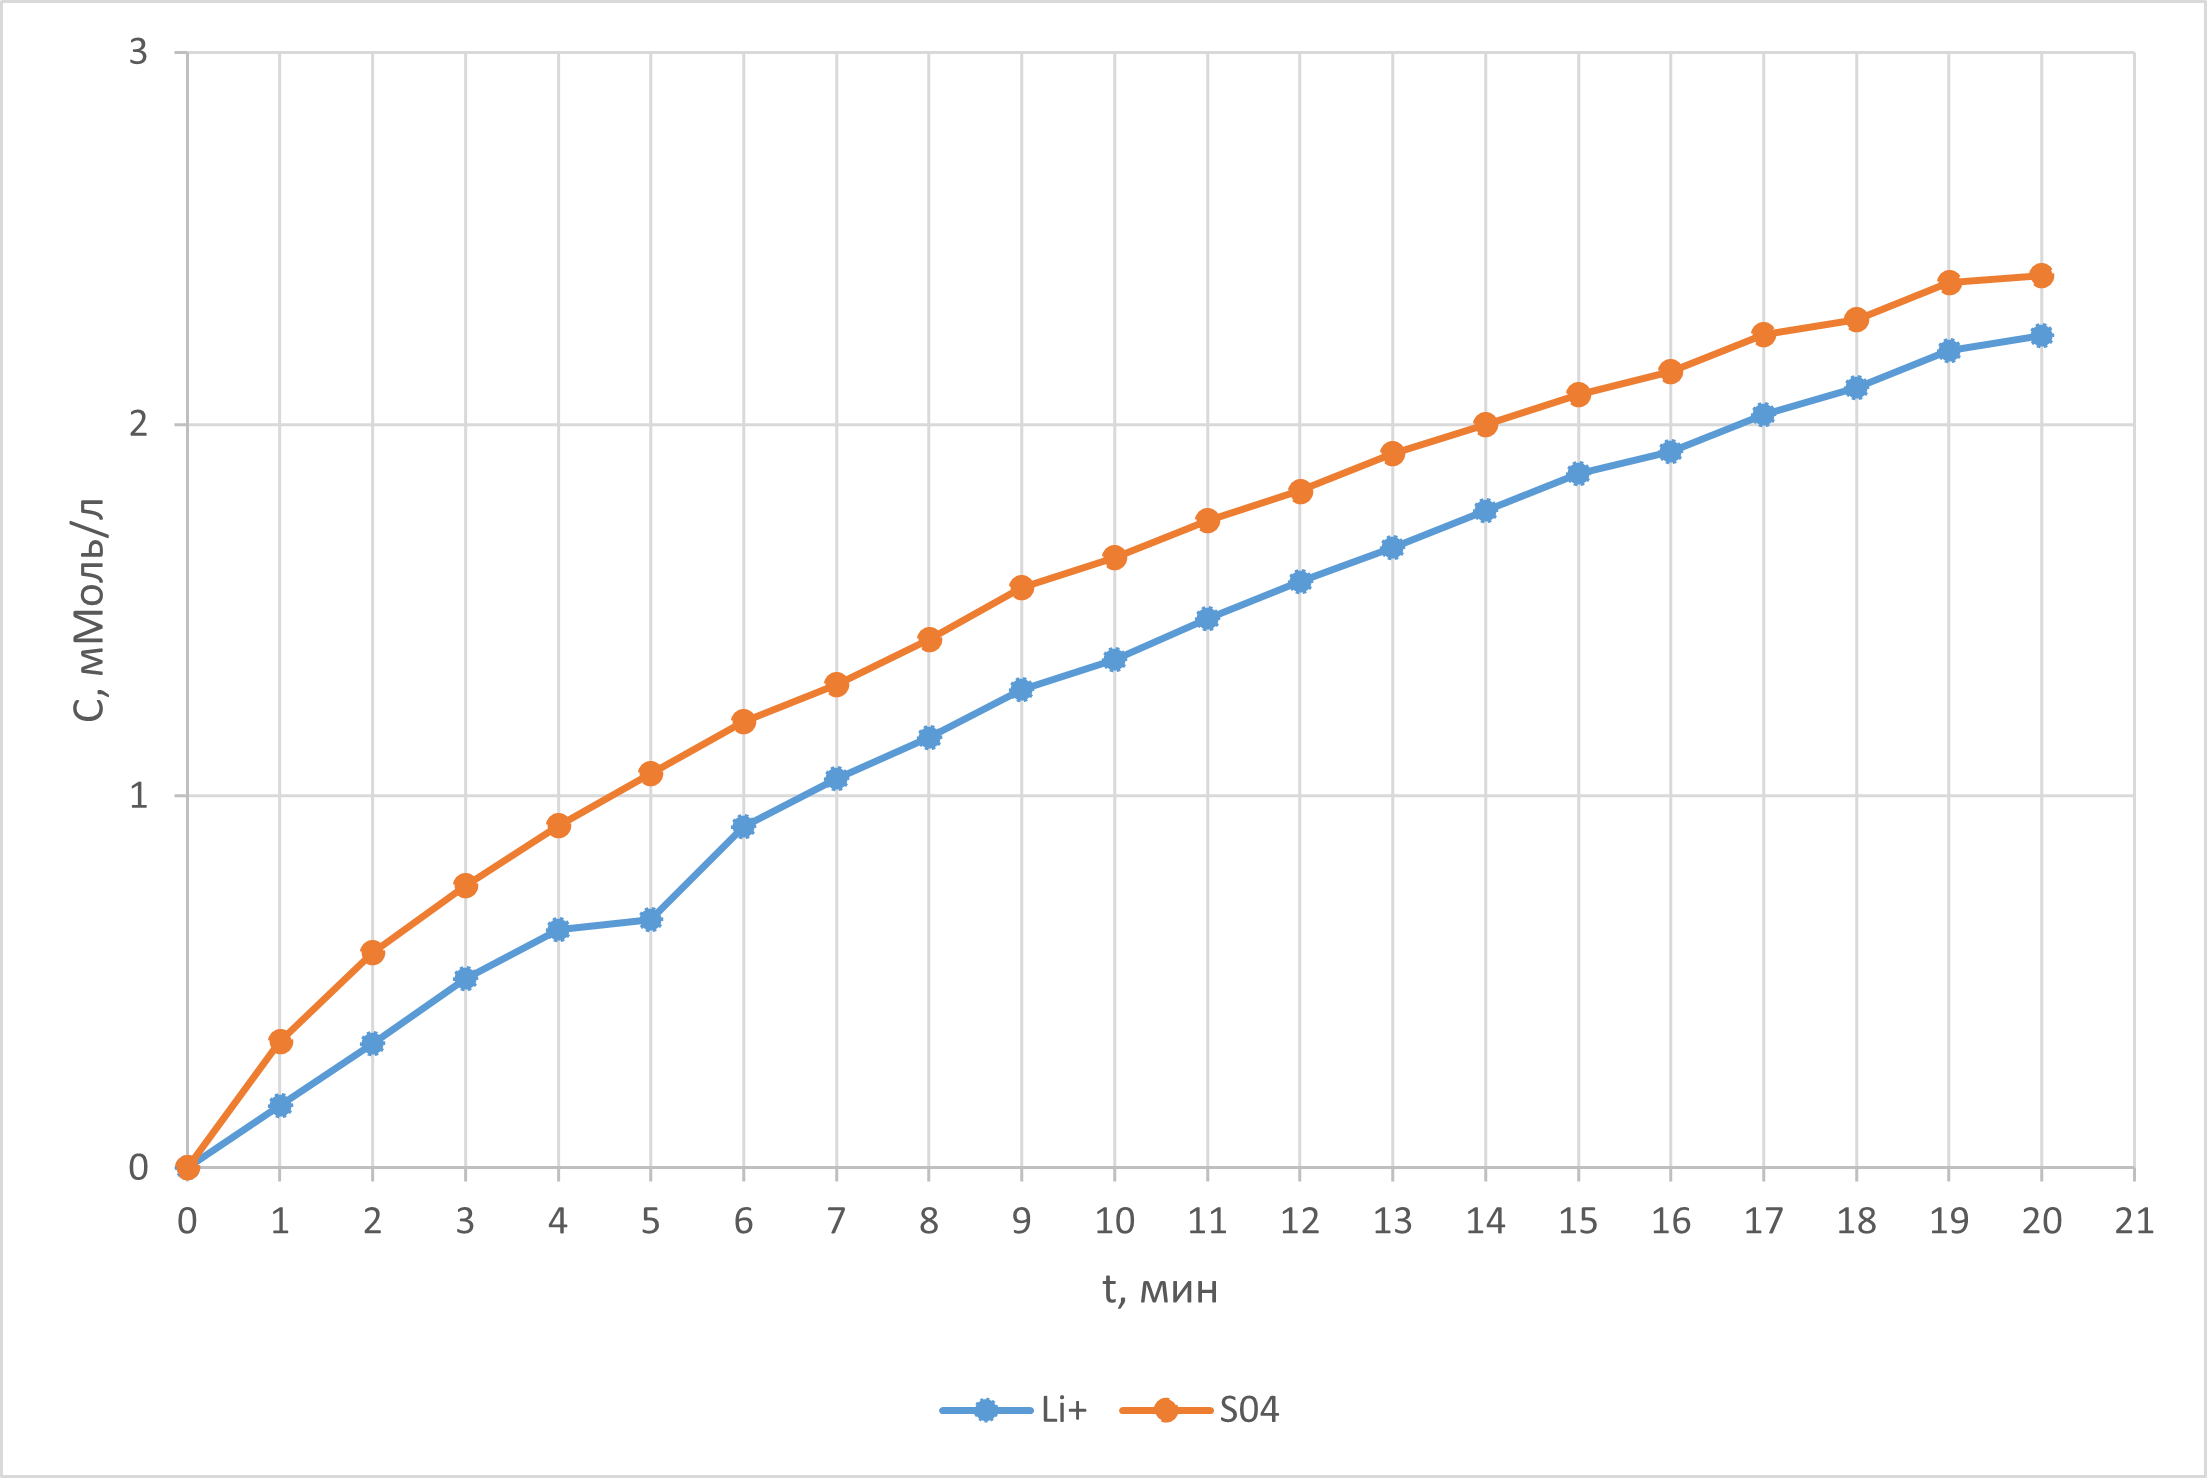
\includegraphics[scale=1]{Рисунок1.png}
    \caption{Кинетическая кривая при pH = 9,5.
}
    \label{pic:1}
\end{figure}

\begin{figure}[H]
    \centering
    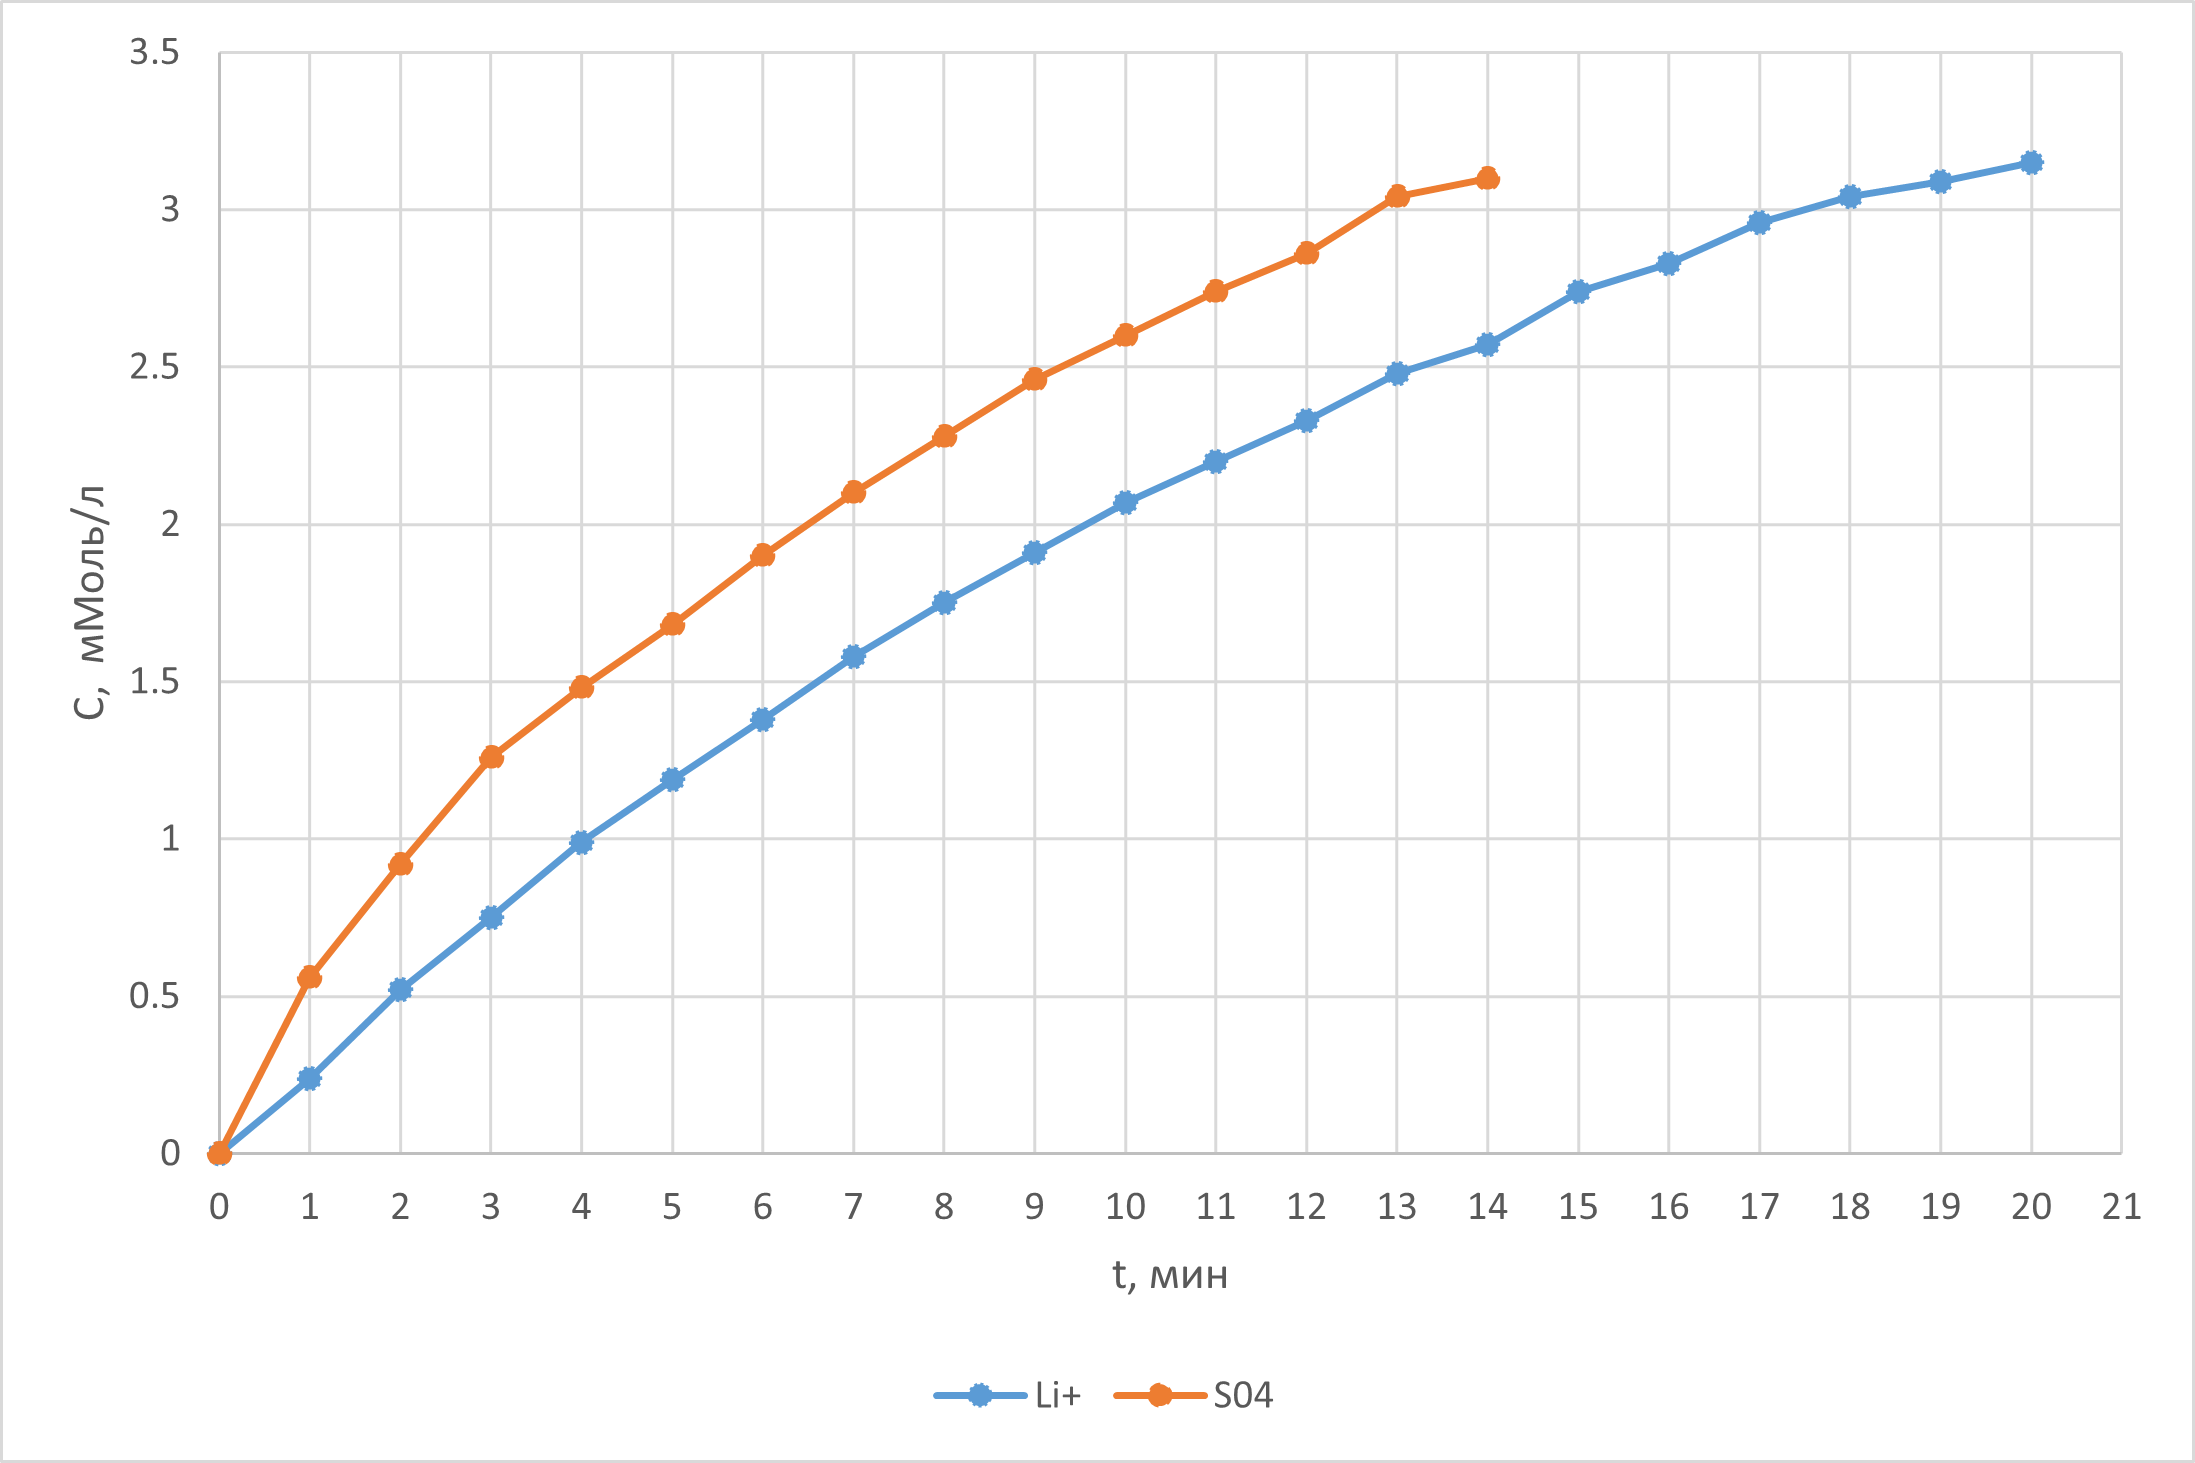
\includegraphics[scale=1]{Рисунок2.png}
    \caption{Кинетическая кривая при pH = 8,5.
}
    \label{pic:2}
\end{figure}

\begin{figure}[H]
    \centering
    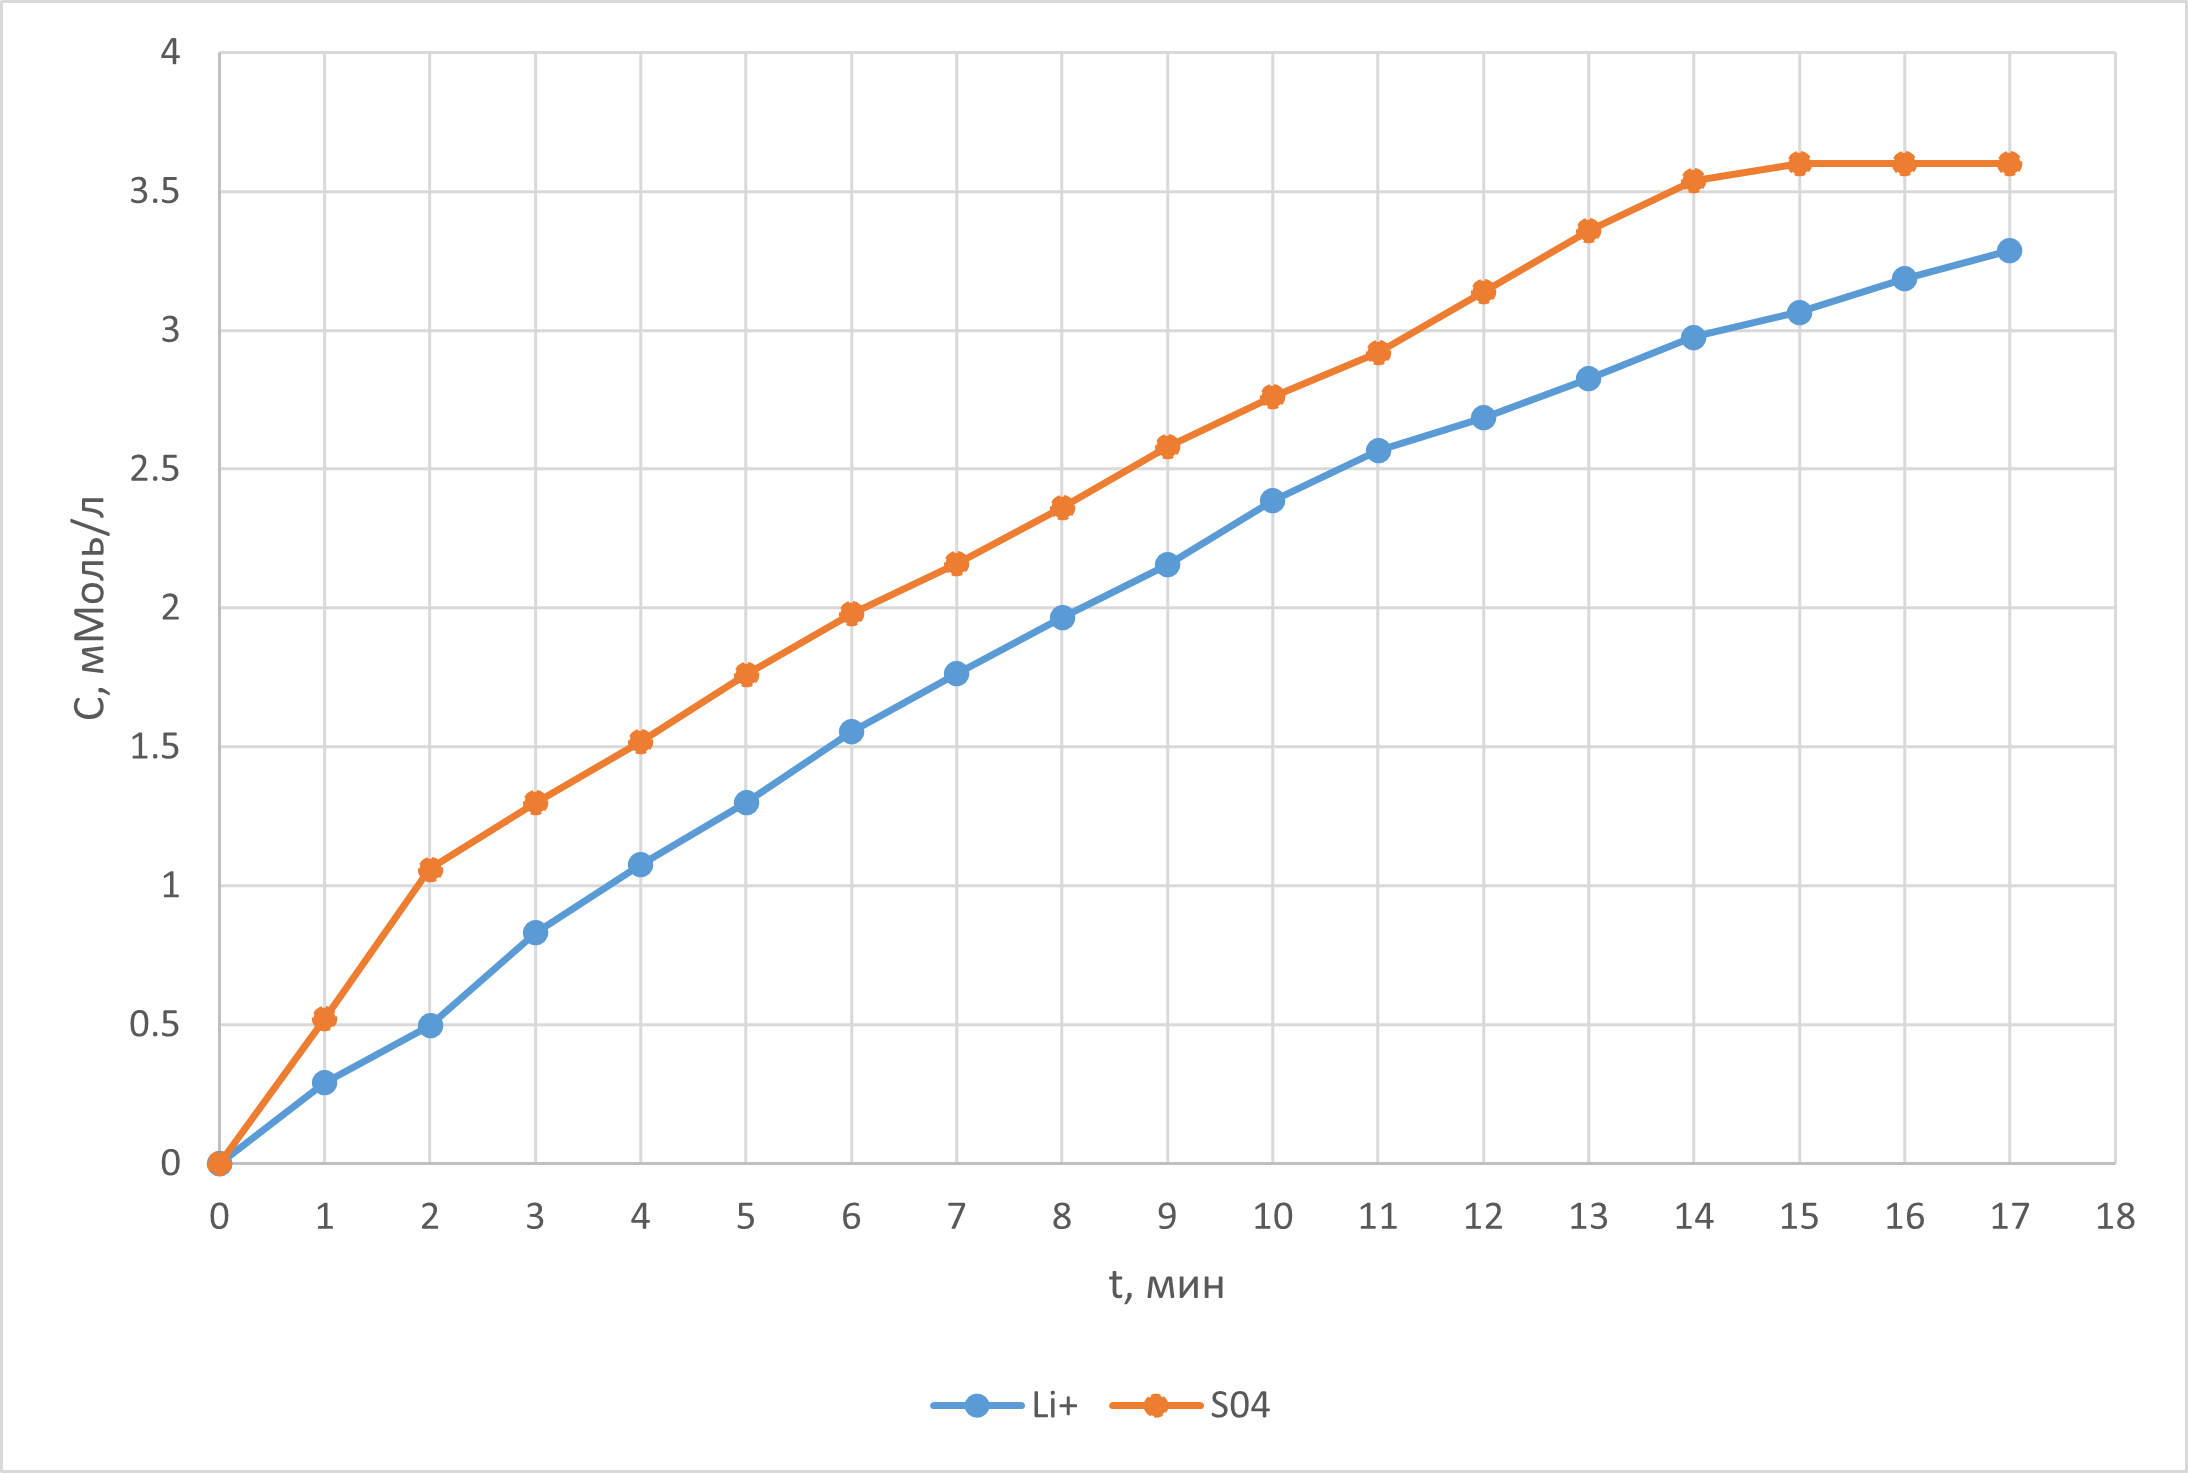
\includegraphics[scale=1]{Рисунок3.png}
    \caption{Кинетическая кривая при pH = 7,5.
}
    \label{pic:3}
\end{figure}

\begin{figure}[H]
    \centering
    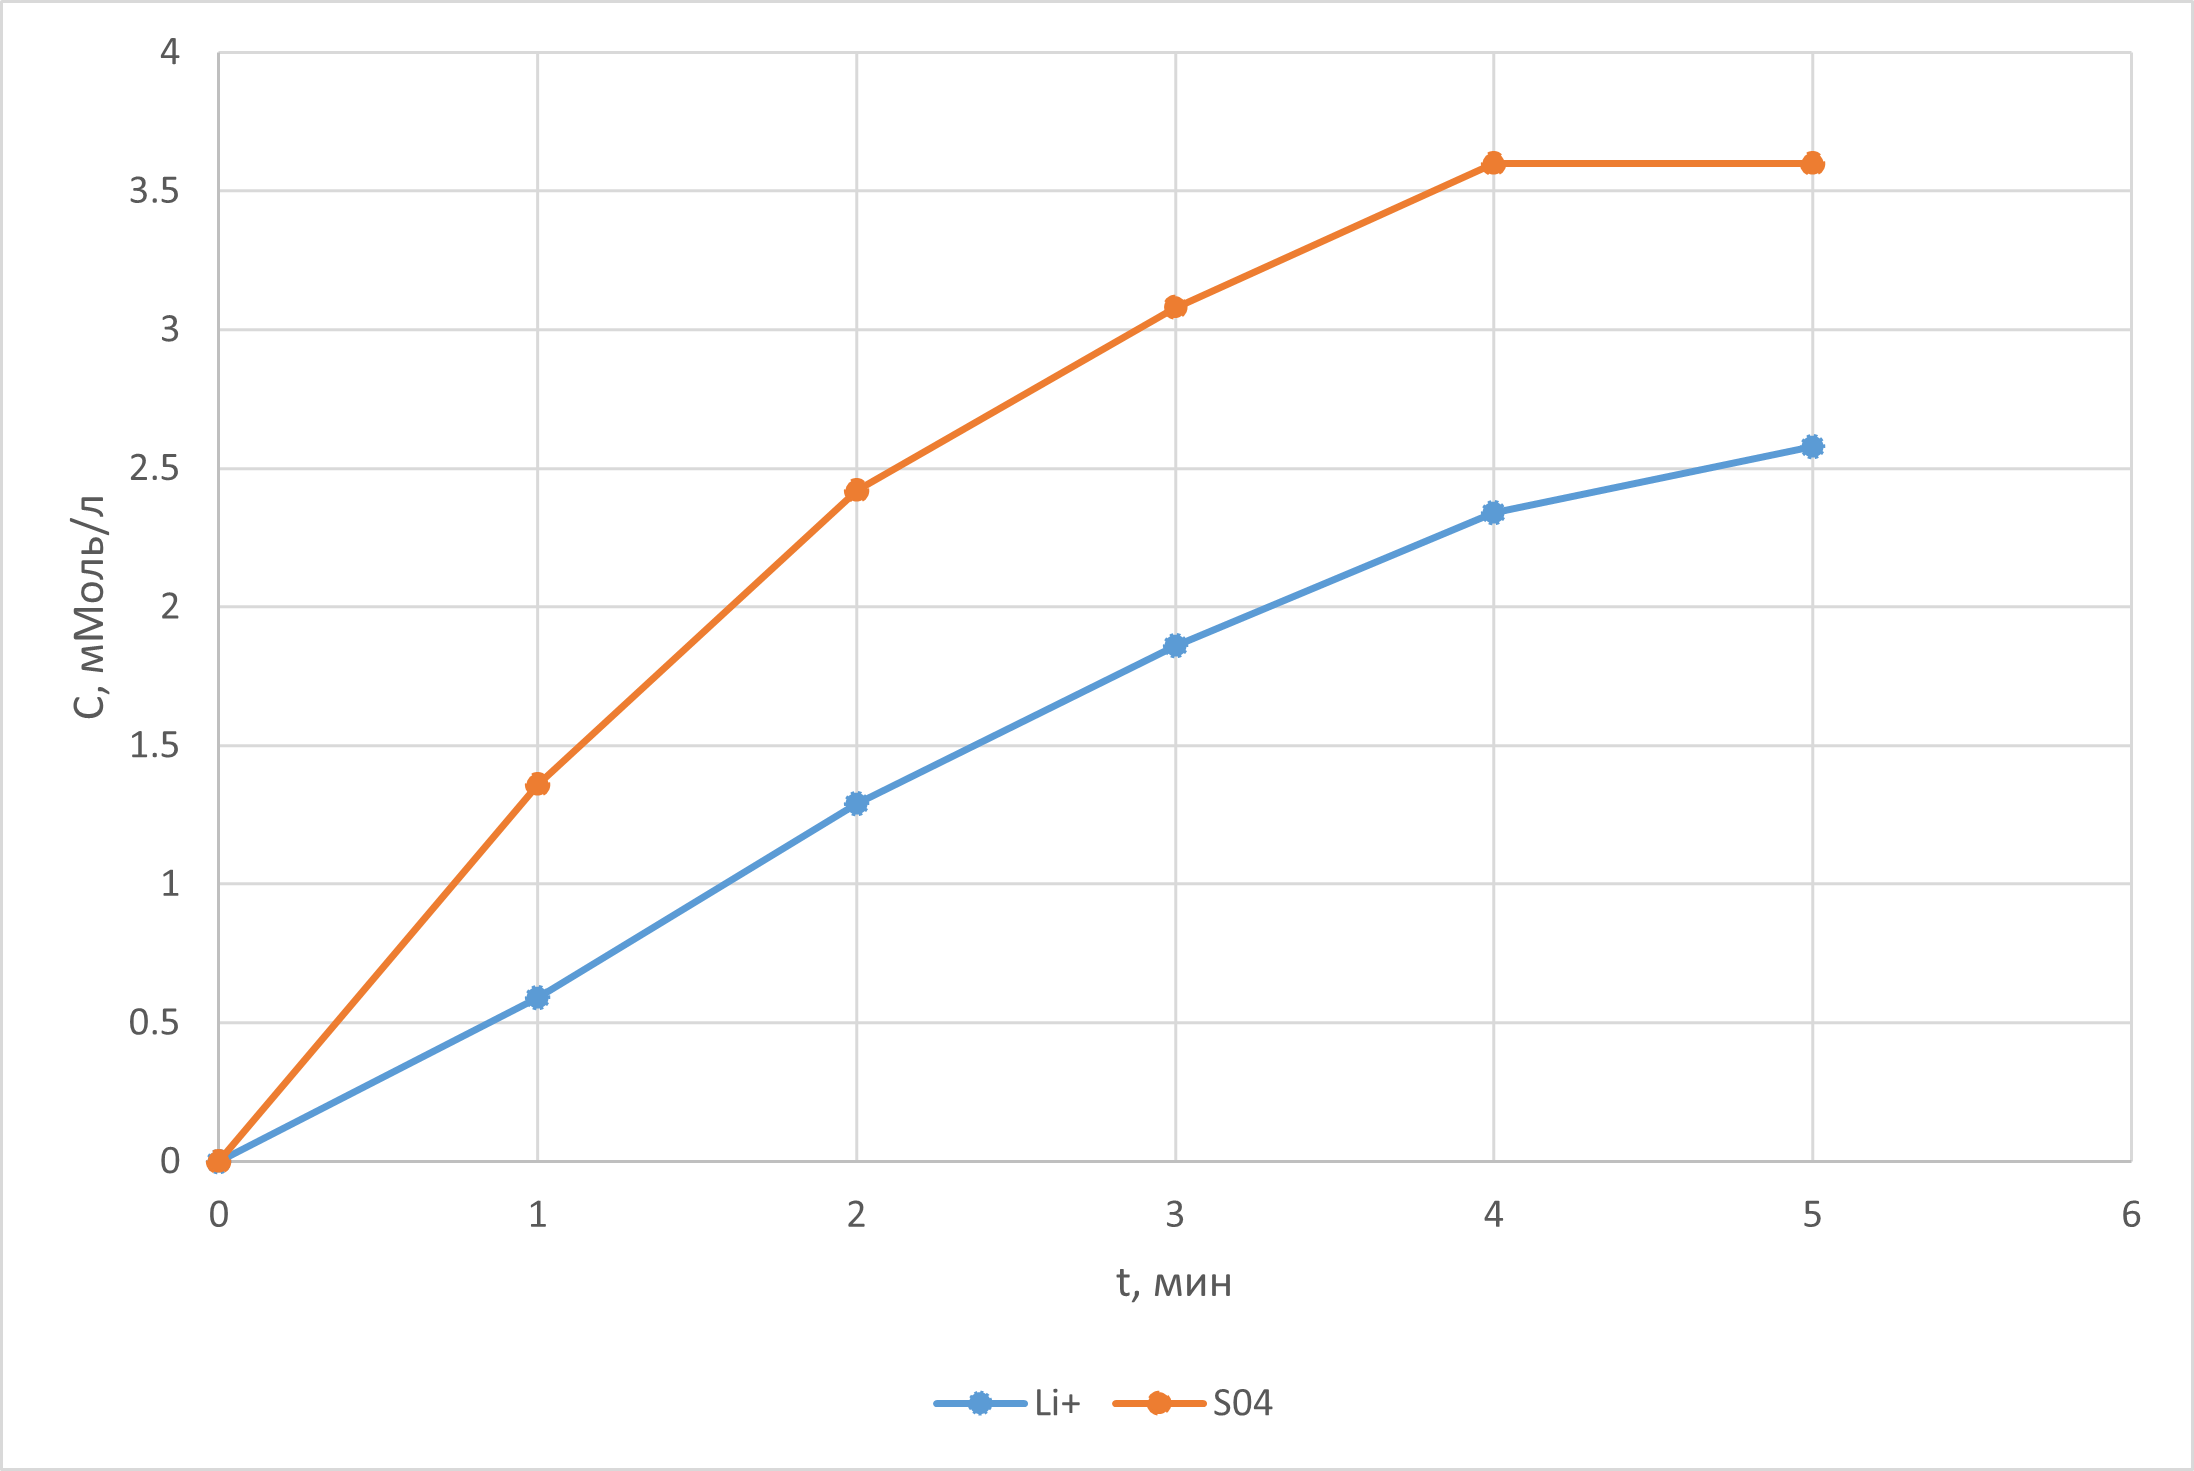
\includegraphics[scale=1]{Рисунок4.png}
    \caption{Кинетическая кривая при pH = 6,5.
}
    \label{pic:4}
\end{figure}


В каждом случае график кинетической кривой ионов лития был ниже, чем аналогичный с хлорид ионами. 

В начале реакции самый большой рост из-за высокой скорости зародышеобразования. Затем отдельные центры реакции (на границе двух твёрдых фаз продукта и реагента) создают сплошной фронт, продвигающийся вглубь твёрдой фазы. Мы не находим перегиба на кинетической кривой, 
что свидетельствует о постоянном замедлении процесса реакции.

Для большей наглядности изобразим так же все кинетические кривые на одном графике.
\begin{figure}[H]
    \centering
    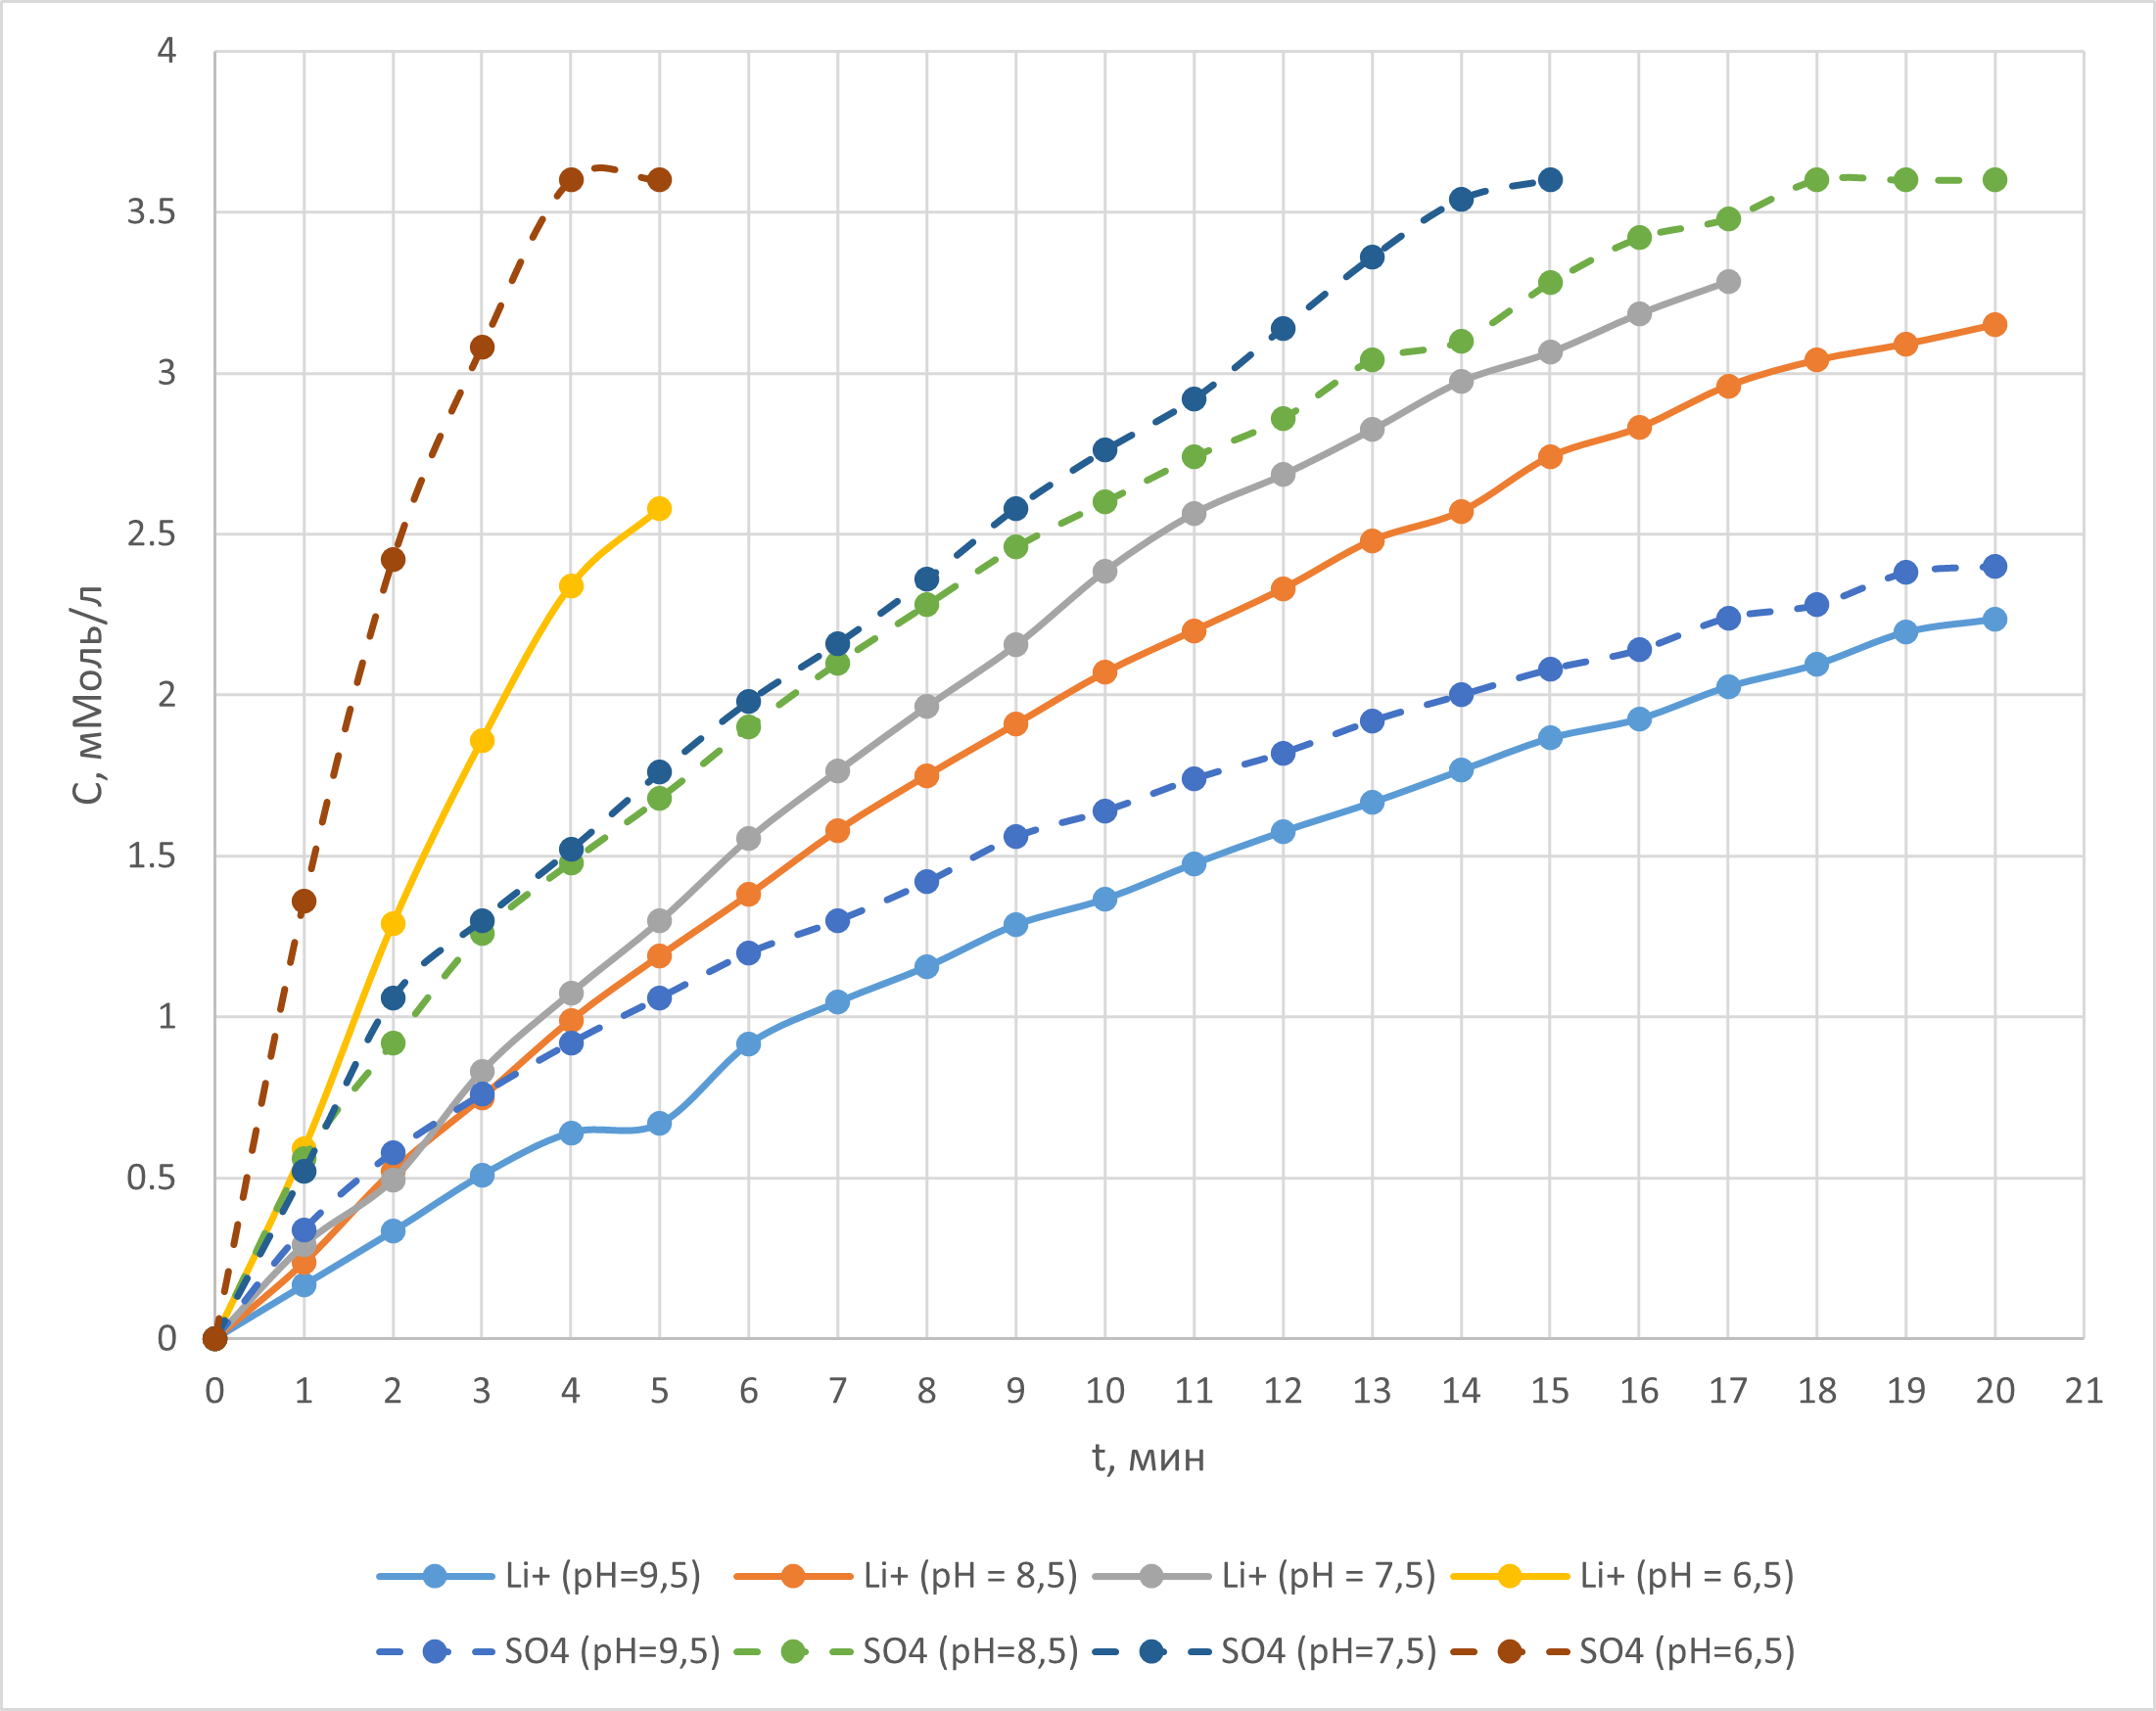
\includegraphics[scale=1]{Рисунок5.png}
    \caption{Все полученные кинетическая кривые
}
    \label{pic:5}
\end{figure}

Наблюдается рост скорости реакции при уменьшении $pH$. Это можно объяснить тем, что в более кислой среде при окислении железа до +3 увеличение числа протонов способствует усилению электростатического взаимодействия между их положительным зарядом и отрицательным зарядом электрона железа (которое может находится в глубине кристаллической решётки вещества, что изначально затрудняет доступ). Тем самым, оторвать электрон у железа легче, что способствует ускорению реакции.

\subsection{Определение степени делитирования}

Определим степень делитирования как $\alpha = \frac{C}{C_0}$, где $C$ - концентрация $Li^+$(мМ) на 10 минуте, $C_0$ = 0,01 М. Значения представлены в таблице \ref{tab:5}. 

\begin{table}[H]
    \centering
    \begin{tabular}{|l|l|l|l|}
    \hline
        $pH$ & 9.5 & 8.5 & 7.5 \\ \hline
        $\alpha$ & 0.14 & 0.21 & 0.24 \\ \hline
        $\alpha, \%$ & 14 & 21 & 24 \\ \hline
    \end{tabular}
    \caption{Степень детилирования $Li^+$ при различных $pH$.}
    \label{tab:5}
\end{table}
Отсюда видно, что степень делитирования увеличивается при возрастании кислотности. Иными словами, выделяется больше ионов лития. 

\subsection{Проверка уравнения Ерофеева-Колмогорова}

Проведём анализ экспериментальных данных по уравнению Ерофеева-Колмогорова \eqref{eq:erof}, где  $\alpha = \frac{C}{C_0}$ - доля прореагировавшего вещества к моменту времени $t$.

Для анализа данных построим график в линеаризованных координатах $ln(-ln(1-\alpha))$ от $ln(t)$. Тангенс угла наклона соответствует значению $n$, пересечение c осью ординат - $lnk$.

\begin{figure}[H]
    \centering
    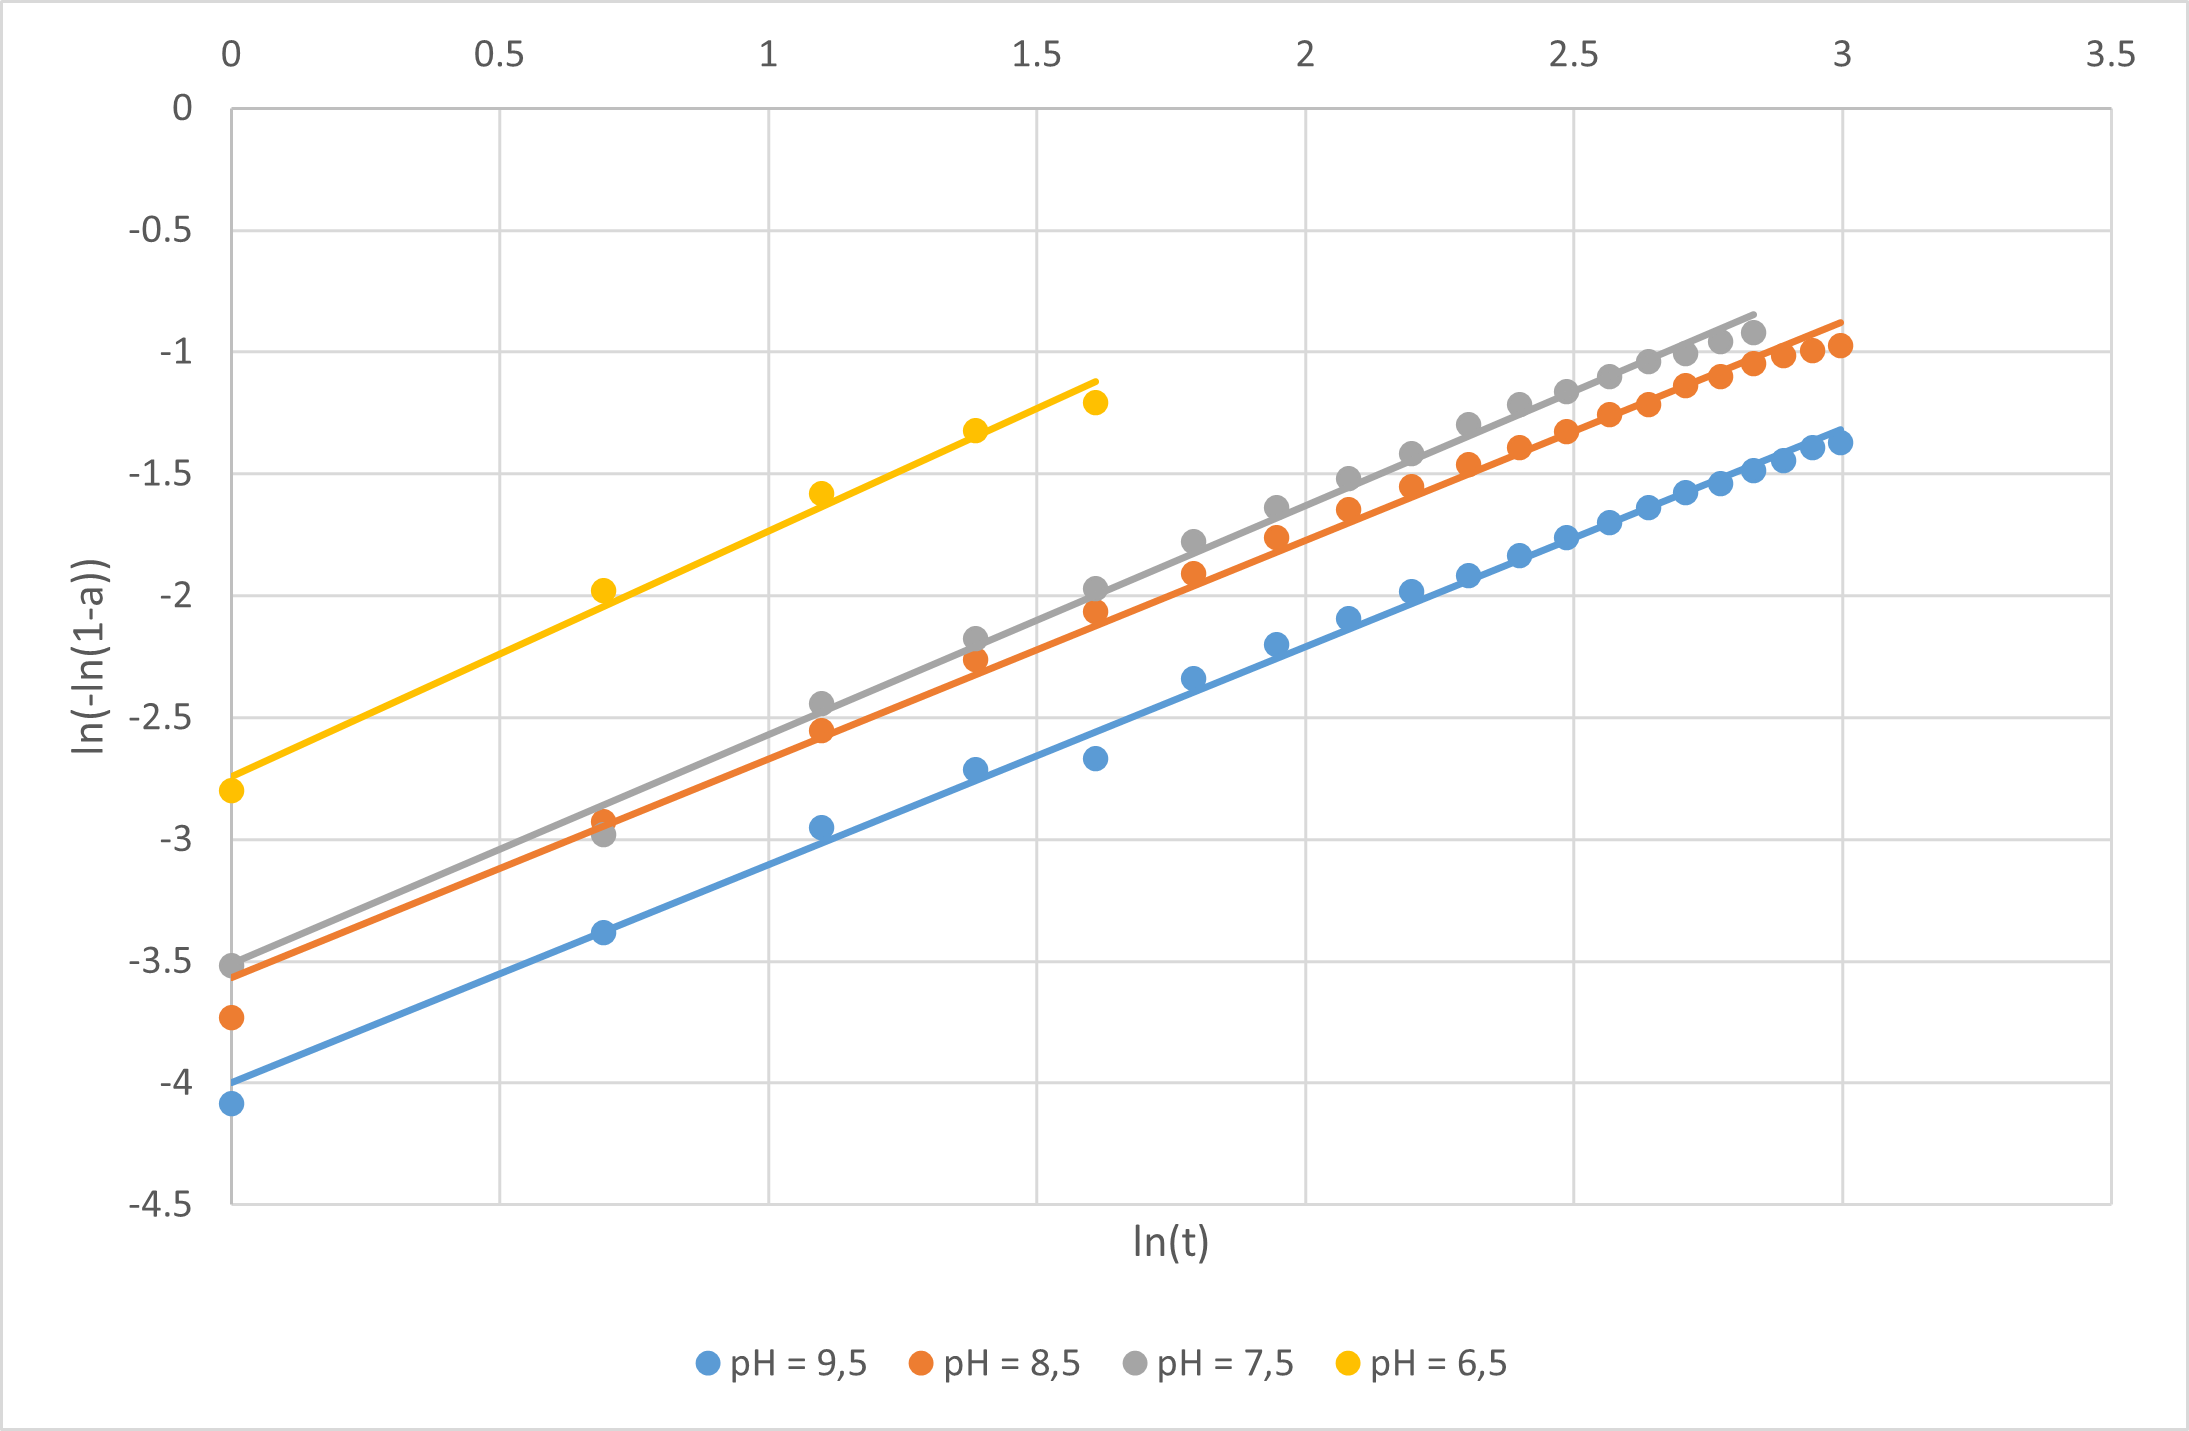
\includegraphics[scale=1]{Рисунок6.png}
    \caption{Проверка уравнения Ерофеева-Колмогорова.
}
    \label{pic:6}
\end{figure}

Видно, что графики аппроксимируются прямой. Сведём результат в таблицу.

\begin{table}[H]
    \centering
    \begin{tabular}{|l|l|l|l|l|}
    \hline
        $pH$ & 9.5 & 8.5 & 7.5 & 6.5 \\ \hline
        $n$ & 0.281 & 0.897 & 0.955 & 1.006 \\ \hline
        $ln(k)$ & -4.084 & -3.73 & -3.519 & -2.8 \\ \hline
        $k$ & 0.017 & 0.024 & 0.030 & 0.061 \\ \hline
    \end{tabular}
     \caption{Определение константы скорости реакции с помощью уравнения Ерофеева-Колмогорова.}
    \label{tab:6}
\end{table}

Если принимать, что точки хорошо аппроксимируются прямыми, то т.к. коэффициент $n<1$ в первых 3-х случаях и $n\approx1$ в последнем, то можно сказать, что лимитирующая стадия диффузионная, то есть происходит либо подвод реагента к частице, либо диффузия вглубь частицы через поры. При увеличении $n$ с ростом кислотности среды процесс переходит в кинетическую область.

\subsection{Проверка уравнения Ленгмюра}
 
Определим константу скорости исходя из уравнения \eqref{eq:leng}. Для этого построим зависимость обратной концентрации ионов лития от обратной величины времени $1/A_t=f(1/t)$. 

\begin{figure}[H]
    \centering
    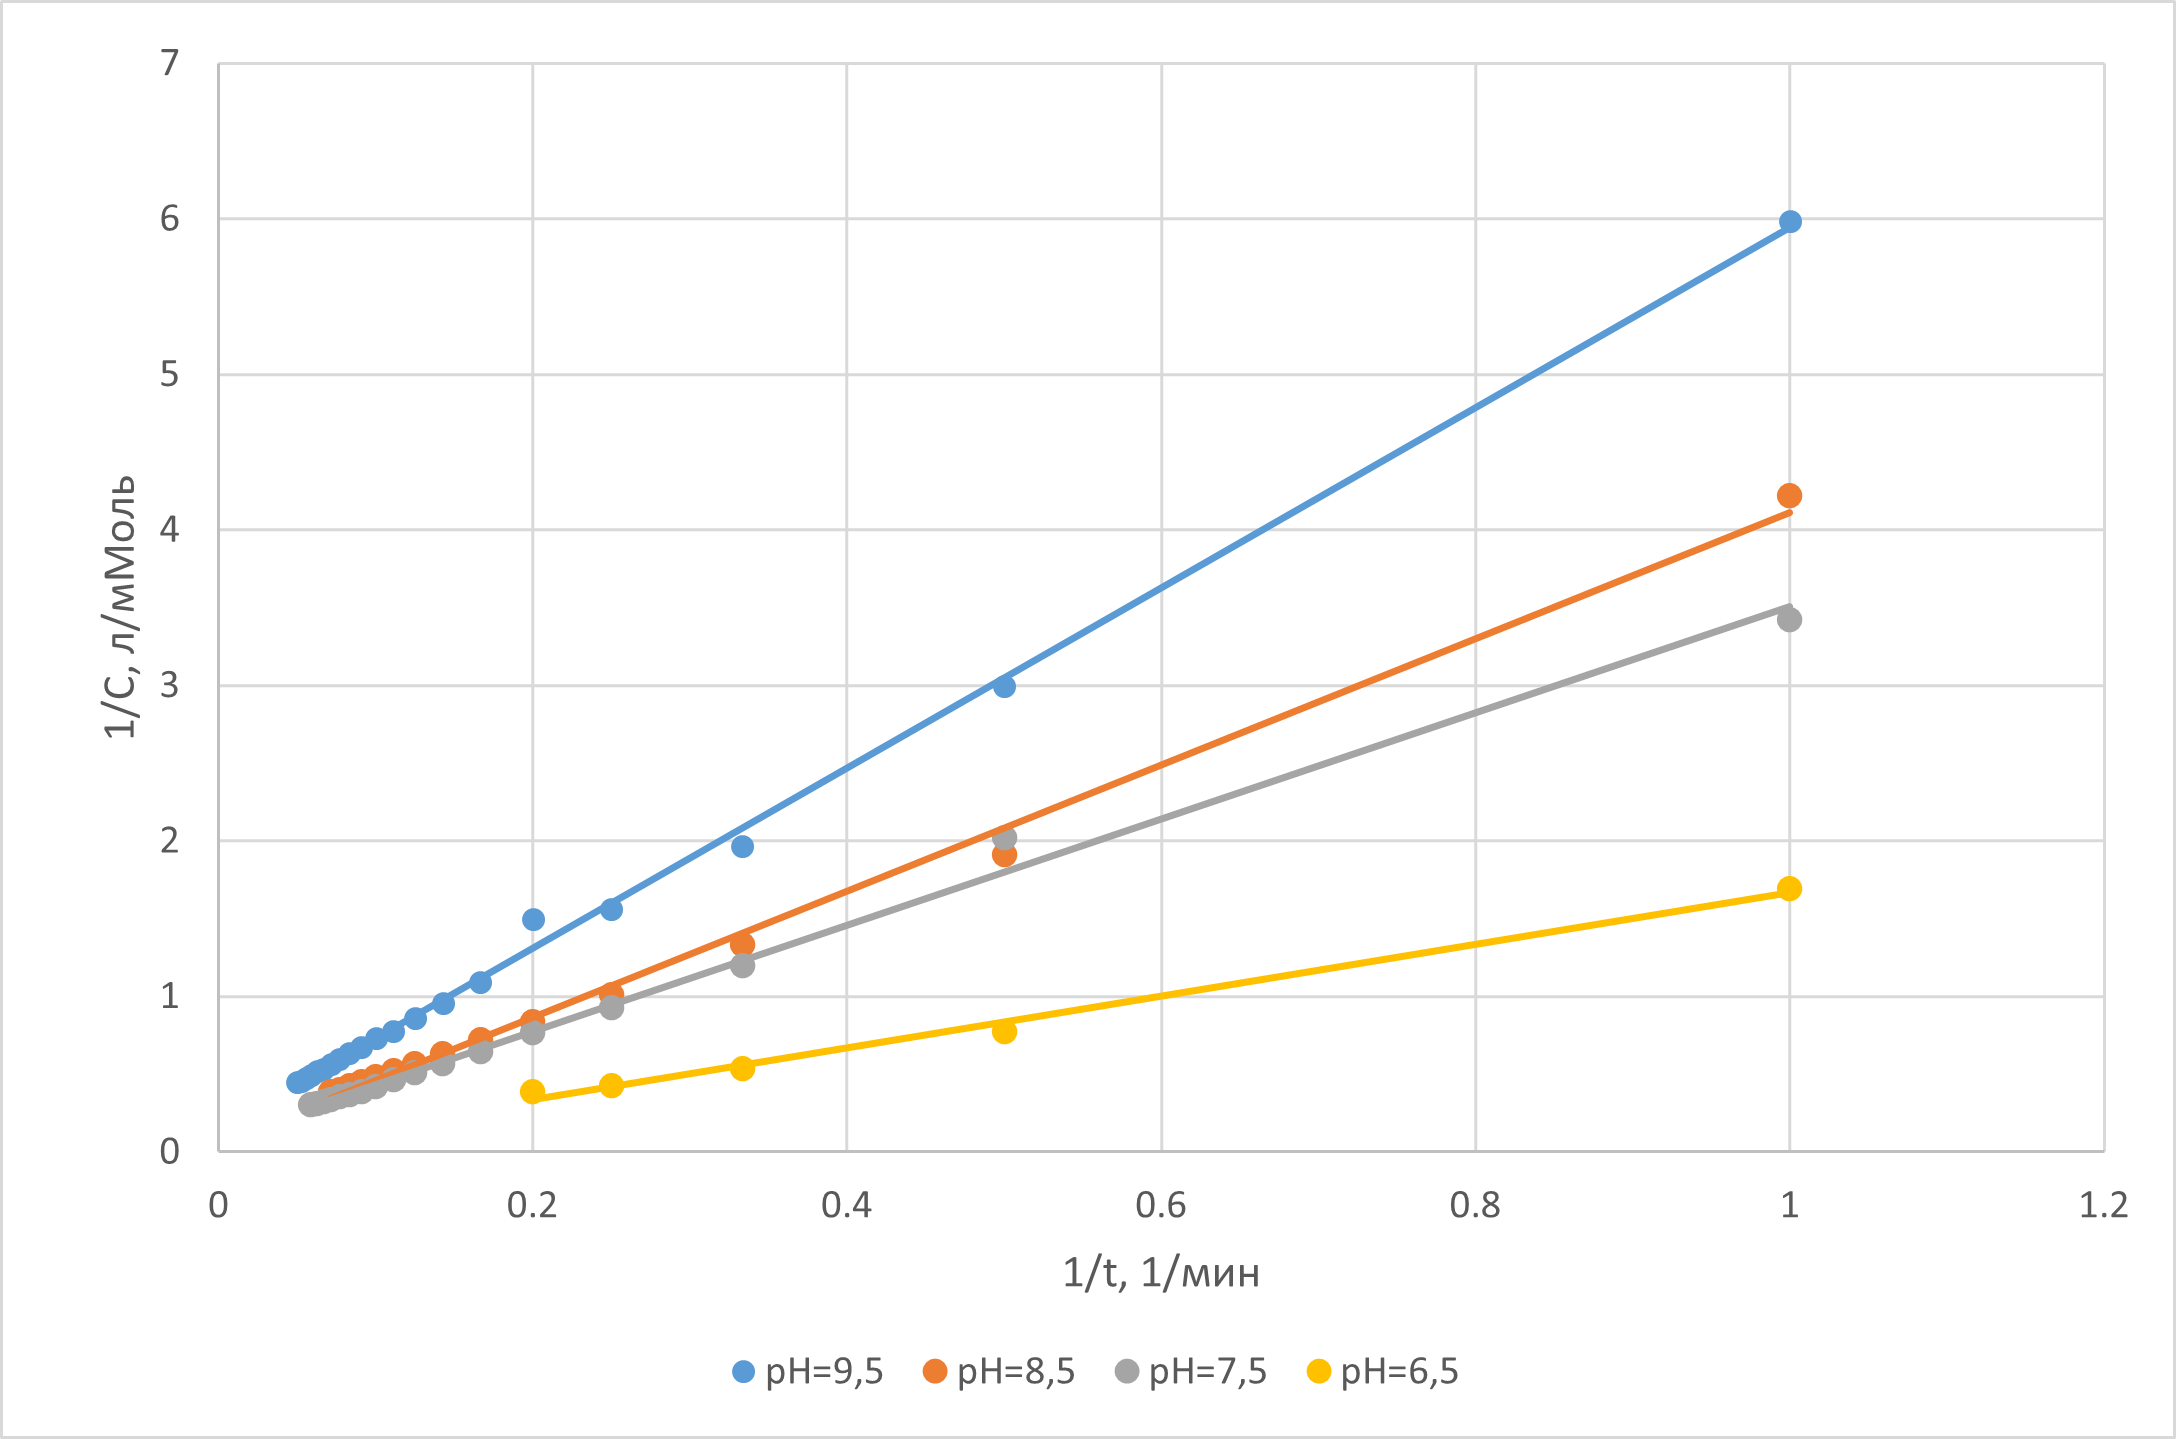
\includegraphics[scale=1]{Рисунок7.png}
    \caption{Проверка уравнения Ленгмюра.
}
    \label{pic:7}
\end{figure}

Результаты тоже хорошо аппроксимируются прямой. Получаемая зависимость $y(x)=ax+b$, где $b=1/A_m, a = 1/kA_m = b/a$. Отсюда посчитаем константу скорости как $k=b/a$ и сведём результат в таблицу.

\begin{table}[H]
    \centering
    \begin{tabular}{|l|l|l|l|l|}
    \hline
        $pH$ & 9.5 & 8.5 & 7.5 & 6.5 \\ \hline
        $a$ & 5.796 & 4.019 & 3.416 & 1.664 \\ \hline
        $b$ & 0.149 & 0.052 & 0.095 & 0.125 \\ \hline
        $k$ & 0.026 & 0.013 & 0.028 & 0.076 \\ \hline
    \end{tabular}
    \caption{Определение константы скорости реакции с помощью уравнения Ленгмюра.}
    \label{tab:7}
\end{table}

\subsection{Зависимость константы скорости от кислотности среды}

Построим графики зависимость $lg(k)$ от $lg([H^+])$, где константу скорости возьмем как среднее из табл. \ref{tab:6} и \ref{tab:7}.

\begin{table}[H]
    \centering
    \begin{tabular}{|l|l|l|l|l|}
    \hline
        $pH$ & 9.5 & 8.5 & 7.5 & 6.5 \\ \hline
        $lg([H^+])$ & -9.5 & -8.5 & -7.5 & -6.5 \\ \hline
        $k$ & 0.0215 & 0.0185 & 0.029 & 0.0685 \\ \hline
        $lg(k)$ & -1.668 & -1.733 & -1.538 & -1.164 \\ \hline
    \end{tabular}
\end{table}

\begin{figure}[H]
    \centering
    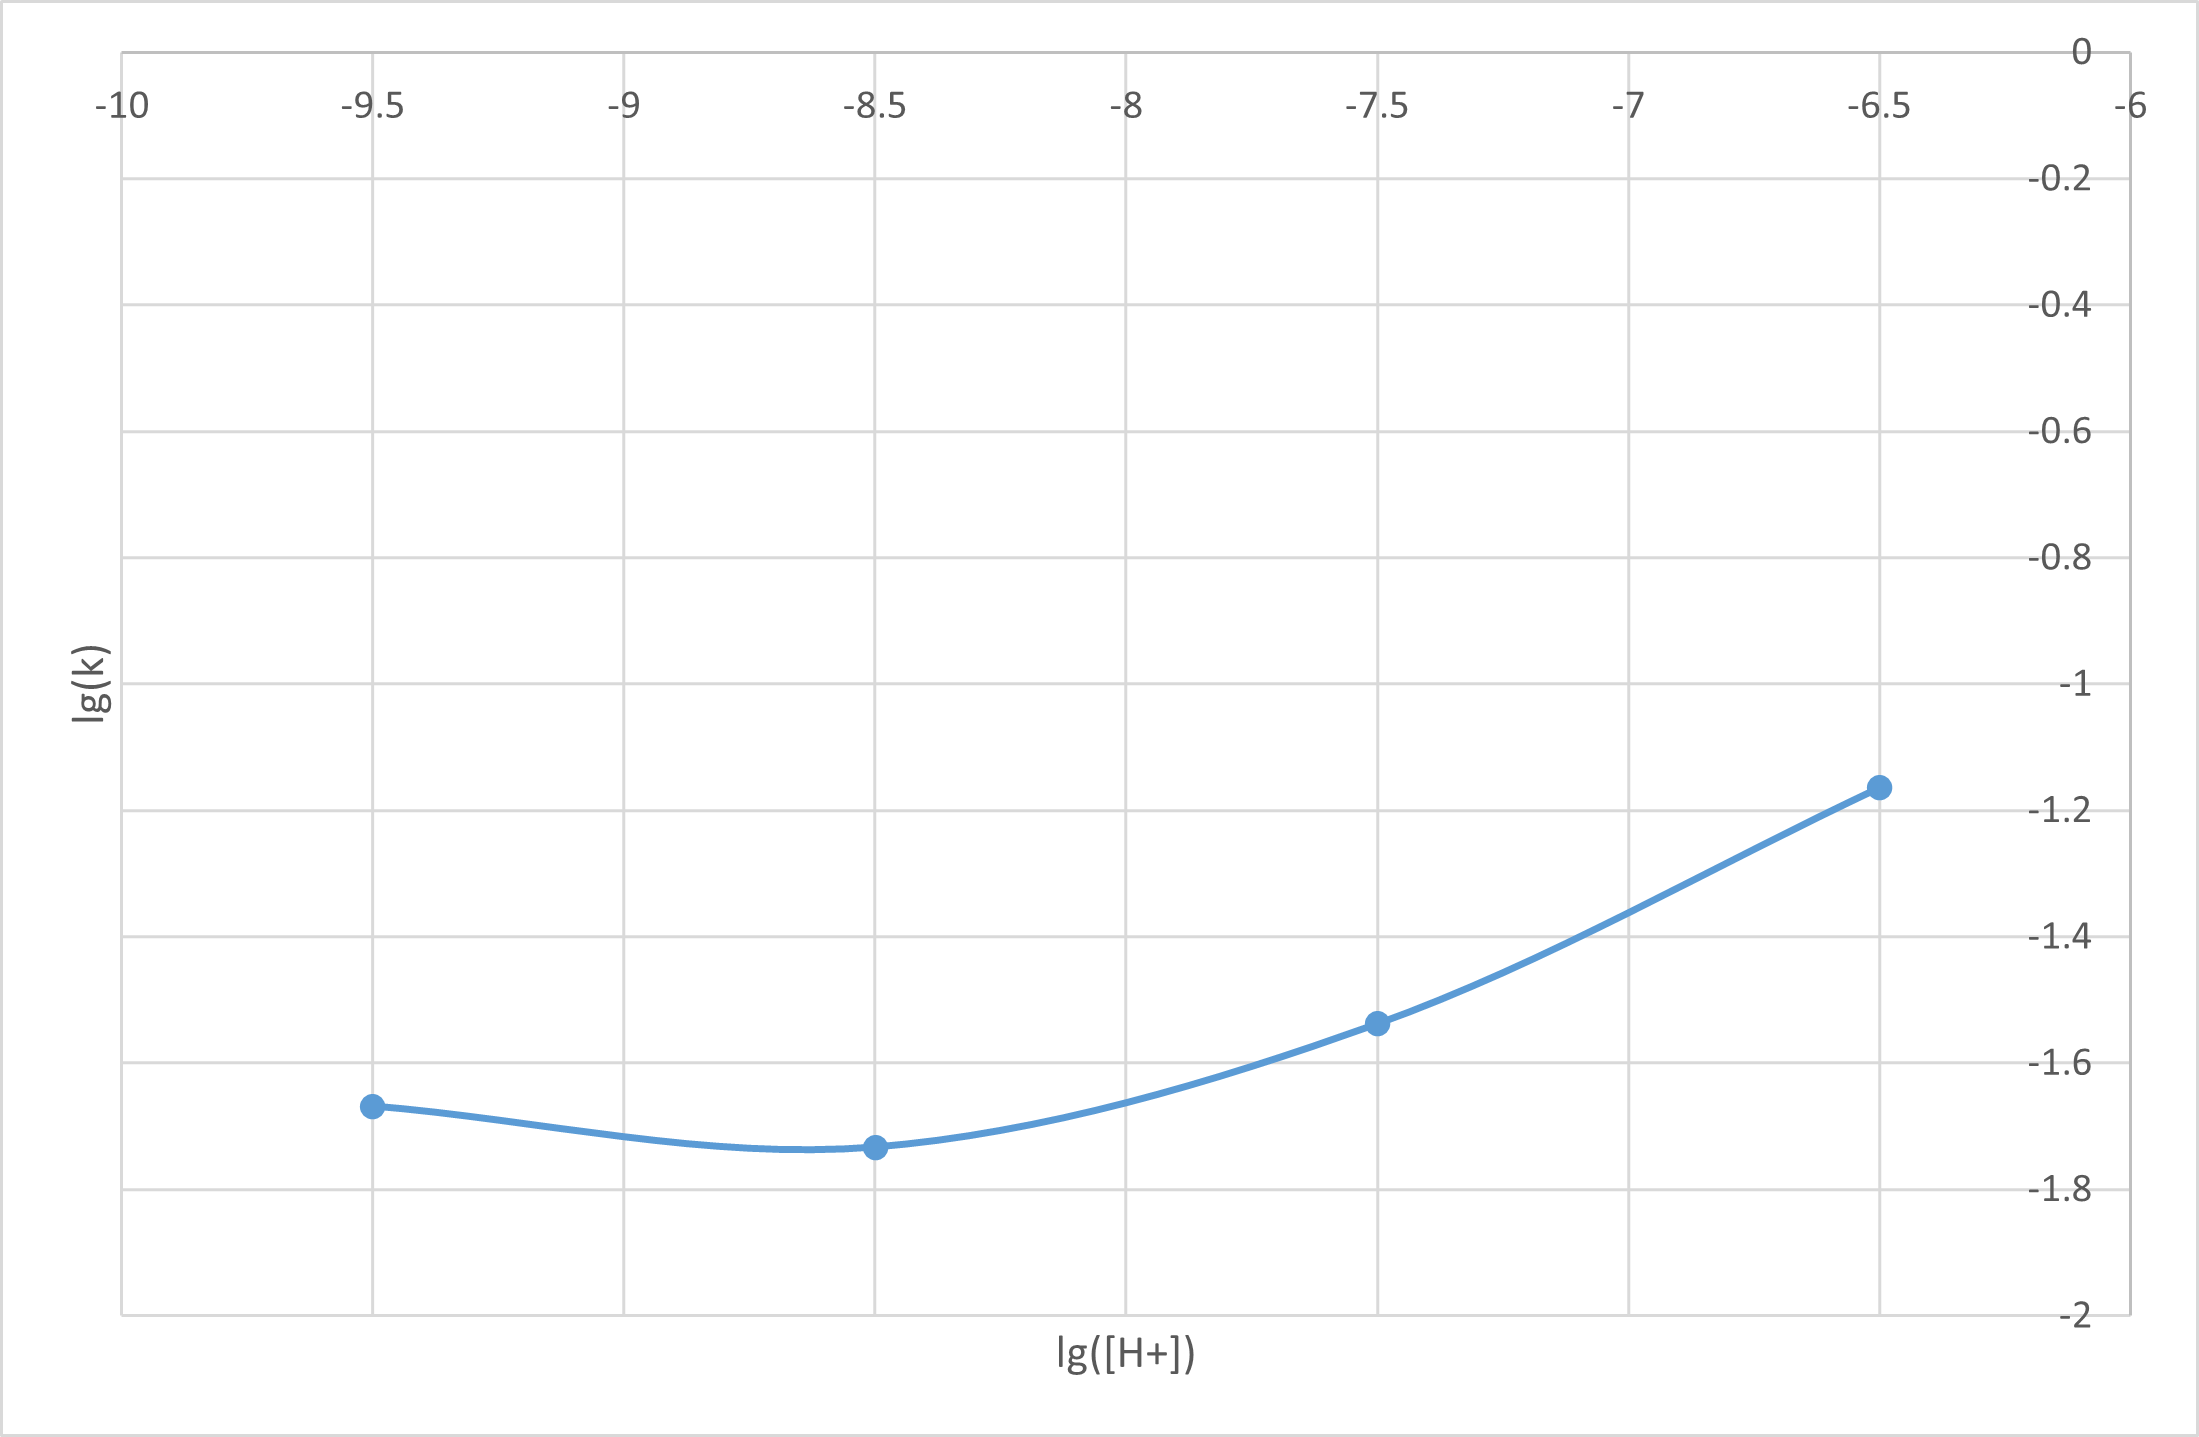
\includegraphics[scale=1]{Рисунок8.png}
    \caption{Зависимость логарифма константы скорости от концентрации протонов.
}
    \label{pic:8}
\end{figure}

Видно, что с увеличением кислотности среды константа скорости возрастает, причем без резких скачков и практически линейно при малых $pH$. 

\section{Вывод}
\begin{itemize}
    \item В ходе работы мы изучили кинетику химического окисления $LiFePO4$ в водной щелочной среде с контролем ионов лития в растворе для определения кинетических характеристик процесса делитирования в зависимости от кислотности среды.
 \item В рамках представлений о топохимических и диффузионно-контролируемых реакциях проанализированы кинетические кривые делитирования $LiFePO4$ (см. рис. \ref{pic:1}, \ref{pic:2}, \ref{pic:3}, \ref{pic:4}). 
\item Используя 2 модели механизма реакции - уравнения Ерофеева-Колмогорова \eqref{eq:erof} и Ленгмюра \eqref{eq:leng} - посчитаны константы скорости, совпадающие по порядку.
\item Из анализа уравнения Ерофеева-Колмогорова (см. рис. \ref{pic:6} и таб. \ref{tab:6}) следует, что лимитирующей стадией в изучаемых процессах является диффузия молекул. 
\item В начале эксперимента модель Ерофеева-Колмогорова описывает исследуемый процесс точнее, чем модель Ленгмюра. В конце эксперимента, напротив, модель Ленгмюра оказывается лучше. Это объясняется тем, что с течением времени расходуются ионы лития на поверхности твердого вещества, а оставшиеся находятся более глубоко, внутри кристаллической решётки, и к этим ионам доступ затруднён остовной структурой. Поэтому в конце эксперимента адсорбция является лимитирующей стадией, именно её и описывает Ленгмюр. А в начале лимитирующей стадией является диффузия. 
\item В заключении можно сделать вывод, что с увеличением кислотности среды скорость реакции увеличивается (см. рис. \ref{pic:5}).
\end{itemize}

\end{document}